 
%\documentclass[]{aa}
%\documentclass[draft]{aa}
%\documentclass[referee]{aa}

\usepackage[varg]{txfonts}

\usepackage{graphicx}

%\usepackage[x11names]{xcolor}
\usepackage{soul}

\usepackage{multirow}	%for tables

\newcommand{\Rs}{$R_\sun{}$}

\usepackage{siunitx}
	\DeclareSIUnit[number-unit-product=\,]\au{au}
	\DeclareSIUnit[number-unit-product=\,]\nT{\nano\tesla}
	\DeclareSIUnit[number-unit-product=\,]\Rs{\textit{R}_\sun{}}
	\sisetup{table-figures-uncertainty=2, table-number-alignment=center, range-phrase=--, range-units=single}



\documentclass[]{aa}
%\documentclass[draft]{aa}
%\documentclass[referee]{aa}

\usepackage[varg]{txfonts}

\usepackage{graphicx}

%\usepackage[x11names]{xcolor}
\usepackage{soul}

\usepackage{multirow}	%for tables

\newcommand{\Rs}{$R_\sun{}$}

\usepackage{siunitx}
	\DeclareSIUnit[number-unit-product=\,]\au{au}
	\DeclareSIUnit[number-unit-product=\,]\nT{\nano\tesla}
	\DeclareSIUnit[number-unit-product=\,]\Rs{\textit{R}_\sun{}}
	\sisetup{table-figures-uncertainty=2, table-number-alignment=center, range-phrase=--, range-units=single}




%AFFECTS
%Promotions-Thema:
%Original:
	%Analyse der Plasma- und Magnetfelddaten des ACE (Advanced Composition Explorer) -Satelliten zur Erstellung von "Echt-Zeit"-Weltraumwetterwarnungen und zur Modellierung solarer Einflüsse auf die terrestrische Ionosphäre im Rahmen des EU FP7 Projektes AFFECTS (Advanced Forecast For Ensuring Communications Through Space).
%Kürzer:
	%Analyse der Plasma- und Magnetfelddaten des ACE-Satelliten zur Erstellung von Echtzeit-Weltraumwetterwarnungen und zur Modellierung solarer Einflüsse auf die terrestrische Ionosphäre im Rahmen von AFFECTS.

	%Analyse von in-situ Sonnenwinddaten zur Erstellung von ``Echtzeit''-Weltraumwetterwarnungen und zur Modellierung solarer Einflüsse auf die terrestrische Ionosphäre.
	
	%Analyse von in-situ Plasma- und Magnetfeld-Sonnenwinddaten - Modellierung der Entwicklung des Sonnenwindes von der Sonne zur Erde und sein Einfluss auf das Erdmagnetfeld zur Erstellung von nahezu Echtzeit-Weltraumwetterwarnungen.

%Original translated:
	%Analysis of plasma and magnetic field data from the ACE (Advanced Composition Explorer) spacecraft for the generation of real-time space weather alerts and for the modeling of solar influences on the terrestrial ionosphere in the context of the EU FP7 project AFFECTS (Advanced Forecast For Communications Through Space).
%Short:
	%Analysis of plasma and magnetic field data from the ACE spacecraft for the generation of real-time space weather alerts and for the modeling of solar influences on the terrestrial ionosphere in the context of the EU FP7 project AFFECTS.

	%Analysis of plasma and magnetic field data from the ACE spacecraft, generation of real-time space weather alerts and modeling of solar influence on the terrestrial ionosphere.

	%Analysis of solar wind plasma and magnetic field in-situ data, generation of near real-time space weather alerts and modeling of the solar influence on the terrestrial magnetic field.
	
	%Analysis of solar wind plasma and magnetic field in-situ data - modeling of solar wind evolution from Sun to Earth and of its influence on the terrestrial magnetic field for the generation of near real-time space weather warnings.
%short:
	%Analysis of solar wind in-situ data - modeling of the solar wind evolution to Earth and of the influence on its magnetic field.
	%Modeling of the solar wind's evolution to Earth and of its influence on the terrestrial magnetic field by analysing solar wind in-situ data.
	

%daraus abgeleiteter Titel in Deutsch:
%Modellierung und Analyse solarer Einflüsse auf die terrestrische Ionosphäre/Magnetosphäre
%Translated titel (topic):
%Modeling and analysis of solar influences on the terrestrial ionosphere/magnetosphere




%daraus abgeleiteter Titel in Deutsch (Version 2):
%Analyse von in-situ Sonnenwind-Messungen zur Erstellung von Echtzeit-Weltraumwetterwarnungen und zur Modellierung solarer Einflüsse auf die terrestrische Ionosphäre...


%SolarProbePlus CGAUSS
%Theme has to be updated, because of SolarProbePlus work...
%Maybe: Analyses of solar wind influence on the terrestrial ionosphere/magnetosphere and modeling of solar wind within the near Sun region

%Analyse der Helios-Datensätze für die Modellierung des Sonnenwindes im Bereich des SolarProbePlus Orbits für die WISPR-Kamera



% maltes_commands.tex
% full journal name replacement
\def\aj{{Astron~.J.}}				%\def\aj{{AJ}}
\def\araa{{Ann~.Rev~.Astron~.Astrophys.}}	%\def\araa{{ARA\&A}}
\def\apj{{Astrophys~.J.}}			%\def\apj{{ApJ}}
\def\apjl{{Astrophys~.J.,~Lett.}}		%\def\apjl{{ApJ}}
\def\mnras{{Mon~.Not~.R~.Astron~.Soc.}}		%\def\mnras{{MNRAS}}
\def\aap{{Astron~.Astrophys.}}			%\def\aap{{A\&A}}
\def\nat{{Nature}}				%\def\nat{{Nat}}
\def\apjs{{Astrophys~.J.,~Suppl~.Ser.}}		%\def\apjs{{ApJS}}
\def\pasp{{Publ~.Astron~.Soc~.Pac.}}		%\def\pasp{{PASP}}

% other short commands
\def\ion#1#2{{\rm #1}{\sc #2}}
\newcommand{\Hi}{\ion{H}{i}}
\newcommand{\Hii}{\ion{H}{ii}}

% new since 2015
\def\planss{{Planet~.Space~Sci.}}		%Planetary and Space Science
\def\grl{{Geophys~.Res~.Lett.}}			%Geophysical Research Letters
\def\ssr{{Space~Sci~.Rev.}}			%Space Science Reviews
\def\jgr{{J~.Geophys~.Res.}}			%Journal of Geophysical Research

% new since 2016-10-20
\newcommand{\Rsun}{$R_\odot$}
\def\solphys{{Solar~Phys.}}			%\def\solphys{{SoPh}}	%Solar Physics
\def\aapr{{Astron~.Astrophys~.Rev.}}		%\def\aapr{{A\&ARv}}	%The Astronomy and Astrophysics Review

% new since 2017-10-05
\newcommand{\Kp}{\textit{Kp}}

% new since 2017-11-04
\def\zap{{Z~.Astrophys.}}			%\def\zap{{ZAp}}	%Zeitschrift für Astrophysik
\def\procspie{{Proc~.SPIE}}			%Proceedings of the SPIE



%\includeonly{filename1,filename2,...}

\begin{document}
	\pagenumbering{Roman}
	
\begin{titlepage}
	\begin{center}
	
	%formelle Titelseite und Rückseite übernehmen.?
	%Unilogo einfügen...
	
		\vspace*{10mm}
		\Large

		%\textbf{Analyses of solar-wind influence\\ \vspace{2mm} on the terrestrial iono-/magnetosphere\\ \vspace{2mm} and modeling of solar wind\\ \vspace{2mm} within the near Sun region}
%Analyses of solar-wind influence on the terrestrial ionosphere/magnetosphere and modeling of solar wind within the near Sun region
		%\textbf{Modeling of the solar wind's evolution to Earth\\ \vspace{2mm}and of its influence on the terrestrial magnetic field\\ \vspace{2mm}by analysing solar-wind in-situ data}
%Modeling of the solar wind's evolution to Earth and of its influence on the terrestrial magnetic field by analysing solar-wind in-situ data.
%		\textbf{Solar wind -- Variability, evolution to Earth\\and influence\\on the terrestrial magnetic field}
		\textbf{Solar wind -- influence on the magnetosphere\\and evolution to Earth} 
		
		\vspace{15mm}
		\large
		Doctoral thesis in physics\\
		\vspace{15mm}
		\textit{Malte~S.~Venzmer}\\
		%aus Stenum?
		\vspace{10mm}
		
		%make cover page image...
		
		\vspace{10mm}

		University of Göttingen\\
		\vspace{5mm}
		Institute for Astrophysics\\
		\vspace{5mm}
		January 2012 -- Jan? 2018\\
		\vspace{15mm}
		Supervisor:\\
		Dr.~Volker~Bothmer\\
		\vspace{5mm}
		Referees:\\
		Prof.~Dr.~Ansgar~Reiners\\
		Prof.~??\\
		
		
	\end{center}
\end{titlepage}

\newpage

\vspace*{5cm}

%Zitat in Diplomarbeit:
%\textit{"[...], und während er sich solchermaßen in der unteren Region des Reiches der Wissenschaft bewegte, dort, wo dieses unmerklich in das Reich der Psychiater übergeht, eignete er sich schließlich doch eine ganze Menge durchaus nützlicher Kenntnisse an, [...]"}
%denn er wusste immer erstaunlich gut Bescheid,
%\noindent Zitat: Stanislaw Lem, "Die Stimme des Herrn", S.56.

%quotes '"``''

\textit{``Despite the `Dr.' before his name, he had completed no course of study and received no degree. When people tried to pin him down about this, he would say that the letters were merely an abbreviation of his first name - Drummond - which he did not use. But it was as `Dr.' Sam Laserowitz that he appeared in a number of science-fiction magazines; he was also known, in the circles of the fans of that genre, as a lecturer, and spoke on `cosmic' themes at their many conferences and convention. Laserowitz's speciality was earthshaking discoveries, wich he happened upon two or three times a year. [...] We really have no idea what a multitude of con men and crackpots inhabit the domain that lies halfway between contemporary science and the insane asylum.''}\\

\noindent Excerpt from Stanis\l aw Lem 1968, \textit{His Master's Voice} \citep[p.~38]{Lem1984}.

%quote vs quotation vs excerpt


\vspace{1cm}

\begin{footnotesize}
\noindent version log:\\
1	2013-11-06\\
2	2013-11-07	inserted lem excerpt\\
3	2014-09-01	outlined introduction structure and appendix key words\\
4	2014-09-11	bibtex included, lem excerpt citet\\
5	2014-09-12	included italic titles in bibliography\\
6	2015-01-12	worked on introduction structure and included magnetic butterfly diagram\\
7	2015-05-04	first printout, small additions\\
8	2015-07-03	coupling functions, content structure\\
9	2015-09-09	Alfv\'en wave velocity formula\\
10	2015-09-10	Appendix physics: Alfv\'en and compressional MHD waves, plasma beta; citation sources Cranmer2005, Kivelson1995\\
11	2015-09-15	CGAUSS work overview; DQCS model figure\\
12	2015-09-16	magnetic energy density is the same as magnetic pressure, abbreviations\\
13	2015-09-30	empirical solar-wind model plots in analyses, figure label [Figure 4.2  Text]\\
14	2015-10-02	table column decimal alignment; set caption width\\
15	2015-10-05	table units; radial parameter (N, T) profiles in literature\\
16	2015-10-06	literature radial electron density models; log-normal distribution\\
17	2015-10-07	log-normal formulae\\
18	2015-10-08	log-normal fit\\
19	2015-10-09	shape fit parameter table; radial variance fitting\\
20	2015-10-14	variance fit values; log-normal citation Bronstein\\
21	2015-10-19	radial distribution width fitting; clarifying of solar-wind model formulae structure and naming variables\\
22	2015-10-20	log-normal distribution width factor changes the shape!\\
23	2015-10-23	log-normal distributions mu and sigma plot\\
24	2015-10-30	new sigmafit2 figures implemented; formulae adaption\\
25	2015-11-02	reason for use of log-normal function\\
26	2015-11-20	single log-normal shape fit; not chisquare - SSR; $R^2$ in appendix\\
27	2015-11-26	reduced SSR into tables; table column aligning\\
28	2015-12-02	smoothing SSR integration\\
29	2015-12-07	integrating structure remarks from printout\\
30	2015-12-09	splitting analyses chapter into two; browsing folders for usable things for thesis\\
31	2015-12-10	integrating citations and references\\
32	2015-12-16	integrating citations and references\\
33	2015-12-18	solar-wind structures list of Richardson\\
34	2016-02-02	sws distributions\\
35	2016-02-11	basics structure\\
36	2016-02-12	analyses questions\\
37	2016-02-15	analyses structure; in situ, near-Sun\\
38	2016-02-16	Kp index internal resolution\\
39	2016-02-17	Bartels1962; non-breaking hyphen shorthand implemented\\
40	2016-02-18	analysesI structure\\
41	2016-02-25	abstract\\
42	2016-02-26	english comma\\
43	2016-03-01	Bartels Kp origin paper, bibtex reference\\
44	2016-03-02	abstract\\
45	2016-03-03	Planck paper\\
46	2016-03-07	formation of stars\\
47	2016-03-08	formation of stars\\
48	2016-03-16	solar interior structure\\
49	2016-03-17	solar interior structure\\
50	2016-03-18	solar surface\\
51	2016-03-22	Astronomical Almanac citation\\
52	2016-03-23	solar core definition\\
53	2016-03-26	sunspots\\
54	2016-03-29	Sun interior figure\\
55	2016-03-30	solar composition\\
56	2016-03-31	Sun interior figure finished; chromosphere\\
57	2016-04-01	Sun atmosphere figure finished\\
58	2016-04-03	chromosphere, corona, CV\\
59	2016-04-07	CV\\
60	2016-04-08	CV; heliosphere\\
61	2016-04-09	corona; heliosphere\\
62	2016-04-11	heliosheath magnetic bubbles; Opher2011\\
63	2016-04-12	heliosphere; voyagers; Gurnett2013\\
64	2016-04-13	solar-wind effects, solar rotation\\
65	2016-04-14	analysesI sws structure draft plots\\
66	2016-04-15	analysesI concept work\\
67	2016-04-19	incorporate annotations from processed printout\\
68	2016-04-21	incorporate annotations from processed printout II\\
69	2016-04-22	incorporate annotations from processed printout III\\
69	2016-04-23	updated .bst file (for displaying arXiv id); implemented optional url displaying for electronic version; Kp year variations\\
70	2016-04-24	Kp frequency by month statistics and plot; Sun and Earth tilt plot\\
71	2016-04-25	solar cycle extrema dates literature\\
72	2016-04-27	Kp semi annual variation, Rangarajan1997\\
73	2016-05-01	Kp frequency by year\\
74	2016-05-04	Kp + SSN plot; ACE data errors/gaps; log-normal plot; differential rotation plot\\
75	2016-05-05	aggregate correlation coefficient tables, CME fraction plot\\
76	2016-05-06	overall sws fractions\\
77	2016-05-17	figure sw frequencies by year; restructured solar-wind distributions section; formal cover page\\
78	2016-05-20	Earth-Sun distance; JPL web interface\\
79	2016-05-31	GSM system\\
80	2016-06-10	Offline Anmerkungen einarbeiten\\
81	2016-06-12	LaTeX Earth symbol package\\
82	2016-06-13	numbers=noenddot\\
83	2016-06-14	references removed comma before ampersand; offline Anmerkungen einarbeiten; thesis\_raw version\\
84	2016-06-17	gnuplot figures and latex; latex document style options\\
85	2016-06-19	header implemented\\
86	2016-06-20	minor things; introduction\\
87	2016-06-23	solar tilt axis\\
88	2016-06-24	solar rotation\\
89	2016-07-12	magnetosphere temp figure; analyses: solar-wind model\\
90	2016-07-13	lognormal spelling\\
91	2016-07-14	constant mass flow rate\\
92	2016-07-18	line-up periods\\
93	2016-07-19	line-up periods table\\
94	2016-07-20	redone line-up analysis\\
95	2016-07-21	line-up tables\\
96	2016-07-22	line-up fit function plots; coefficient table\\
97	2016-07-22	line-up sw types and period plots; overview plot\\
98	2016-07-24	line-up averaging and justification\\
99	2016-07-29	line-up rework\\
100	2016-07-30	line-up structure\\
101	2016-07-31	line-up table\\
102	2016-08-02	line-up structure\\
103	2016-08-03	line-up fits and table\\
104	2016-08-04	insert offline comments\\
105	2016-08-15	literature radial sw functions\\
106	2016-08-18	work offline comments in\\
107	2016-08-19	work offline comments in\\
108	2016-08-28	analyses II rework structure\\
109	2016-08-31	analyses II rework structure\\
110	2016-09-01	analyses II rework figures\\
111	2016-09-02	analyses II rework structure\\
112	2016-09-03	Helios latitude dependency\\
113	2016-09-04	extrapolation model fit parameter table; Helios latitude dependence\\
114	2016-09-06	work in offline comments\\
115	2016-09-14	implement median and mean in composite fit table; create kile project for thesis; url and raw fork\\
116	2016-09-17	Ulysses polar plot; solar distance plots\\
117	2016-09-18	for solar distance and latitude -> 4-panel figures created and implemented; appendix figures\\
118	2016-09-20	latitude plots updated\\
119	2016-09-26	single lognormal fit figure\\
120	2016-09-27	minor tweaks in analyses II\\
121	2016-09-29	simple fit table errors; table style\\
122	2016-10-05	lognormal fit errors for tables\\
123	2016-10-10	line-up passing remarks from AP\\
124	2016-10-12	siunitx package incorporated\\
125	2017-01-04	package fancyhdr replaced with scrlayer-scrpage; offline comments for Basics + Data incorporated\\
126	2017-01-06	package floatrow included for figure side captions; some cites; magnetometer\\
127	2017-01-08	sun figure updates and new ion energy spectrum figure incorporated\\
128	2017-01-13	offline comments, new chapter order\\
129	2017-01-18	activated hyperref package; included autoref and eqref; adjusted link colors; header links\\
130	2017-02-02	offline commtents\\
131	2017-02-03	offline commtents II, eclipse image\\
132	2017-02-06	basics figures with floatrow; flow structure\\
133	2017-02-07	ion energy spectrum figure\\
134	2017-02-09	Helios mission ssn plot\\
135	2017-02-12	offline comments\\
136	2017-02-13	section number link to toc; offline comments\\
137	2017-02-14	eclipse and magbfly figure captions\\
138	2017-02-16	offline comments\\
139	2017-02-19	coronal heating and sw acceleration\\
140	2017-04-22	set up git repository\\
141	2017-04-23	incorporate offline comments\\
142	2017-04-26	bipolar region draft\\
143	2017-04-27	magnetic layer Ossendrijver2003\\
144	2017-06-29	magnetosphere figure drafts implemented\\
145	2017-07-16	streamlined content - including paper and chapter2\\
146	2017-07-22	streamlined duplicate content\\
147	2017-10-05	Kp index data\\
148	2017-10-28	geomagnetic indices; Kp index; Kp to ap table\\
149	2017-10-29	Kp index\\
150	2017-10-30	OMNI s/c coverage figure\\
151	2017-10-31	OMNI s/c coverage figure upgrade; data set timeline figure\\
152	2017-11-01	SSN prediction; omega-effect\\
153	2017-11-02	alpha-omega dynamo; magnetogram figure upgrade\\
154	2017-11-03	worked on figure permissions; alpha-omega-figure\\
155	2017-11-04	paperMVVB inserted; worked on compatibility\\
156	2017-11-12	paperMVVB: figure size, tablefoot, adjusted table width; included chapter2; ordered file implementing\\
157	2017-11-14	figure permission Babaszkiewicz1998\\
158	2017-11-15	poking around in image credits; solar activity cycle\\
159	2017-11-16	solar activity cycle; Zhao image permission\\
160	2017-11-17	Zhao copyright symbol included; solar-wind; commata and sentence wording\\
161	2017-11-22	notes from github paper folder\\
162	2017-11-23	Ulysses figure permission and caption; pdfpages package; paper included as is\\
163	2017-11-24	GUM reference; Helios data frequency figure\\
164	2017-11-25	intro to paper\\
165	2017-11-26	intro to paper\\
167	2017-11-27	Cranmer2005 fig1; Banaszkiewicz fig\\
168	2017-11-28	HCS and Parker spiral\\
169	2017-11-29	heliosheath; Cranmer2005 permission\\
170	2017-11-30	chapter2 updated\\
171	2017-12-06	upgraded: title, abstract, introduction, basics outline, notes to chapter2; worked in offline comments until HMF\\
172	2017-12-08	MBPs; Solar wind section structure\\
173	2017-12-10	solar wind basics, draft figs for CIR and CME\\
174	2017-12-11	draft figs for COR2 CME and ACE MC; solar wind history\\
175	2017-12-13	B-field improvement\\
176	2017-12-14	B-field improvement \#2\\
177	2017-12-15	B-field improvement \#3\\
178	2017-12-16	B-field angles plot\\
179	2017-12-17	B-field improvement \#4\\
180	2017-12-21	B-field: four plots upgraded\\
181	2017-12-31	B-field: worked offline comments in; included chapter2 update\\
182	2018-01-01	autoref names; solar wind properties; literature\\
183	2018-01-02	sw helium share; plasma beta; source surface; mass flux considerations\\
184	2018-01-04	sw considerations; fast/slow wind\\
185	2018-01-05	fig Hundhausen; fast slow sw\\
186	2018-01-08	fast slow sw\\
187	2018-01-09	slow sw sources\\
188	2018-01-10	slow sw; slow/fast cycle pattern\\
189	2018-01-11	Wang1990\\
190	2018-01-14	HCS and SIR\\
191	2018-01-15	HCS + CIR\\
192	2018-01-16	in-situ event plots\\
193	2018-01-17	in-situ CIR/HSS plot\\
194	2018-01-19	CME/MC plot; VB comments\\
195	2018-01-20	VB comments\\
\\
\ISOToday{} \thistime{} -- last save
\end{footnotesize}

\newpage

%\abstract
\begin{abstract}
\section*{Abstract}
This thesis analyzes how strong the solar wind and its internal structures impact the terrestrial magnetosphere and how the solar wind evolves on its way from the Sun.
%magnetosphere impact
In situ solar-wind measurements from the near-Earth OMNI data set are analyzed together with time series of the planetary geomagnetic disturbance indicator \Kp{}. Correlation functions are compiled with regard to nowcast the magnitude of the geomagnetic disturbances from solar-wind measurements and to forecast them from remotely observed streams and CMEs.
%solar activity
In situ data from the near-Earth OMNI data set and sunspot number data is used for deriving functional dependences with the state of the solar cycle for the solar-wind parameters magnetic field strength, proton velocity, density, and temperature.
%solar distance
Data from the Helios~1 and 2 missions is analyzed and empirical solar-wind distance dependencies for \SIrange{0.3}{1.0}{\au} are derived. Additionally, in view of the planned near-Sun spacecraft mission Parker~Solar~Probe (PSP), the solar-wind environment is estimated down to \num{<10}~solar radii.\\

catch from chapter abstracts...\\

%key words: solar wind; sun: corona; sun: heliosphere; Parker Solar Probe (PSP); magnetosphere; Kp index\\
%German title:\\
%german abstract: Kurzfassung\\
\end{abstract}

%\cleardoublepage
%\tableofcontents
{\let\cleardoublepage\clearpage\tableofcontents}	%open contents on left page
\label{toc}
%\listoffigures
%\listoftables

		%cover_formal
	\pagenumbering{arabic}
	
\chapter{Introduction}
\label{chap:introduction}

%Kurzer Text zur Motivation für diese Arbeit; wie es zum Thema kam und wie das Ziel erreicht wurde

Introductory text -> motivation\\
- \Kp{} impact analysis\\
- solar activity analysis\\
- distance analysis\\

% Questions this work asks:\\	%Fragestellungen ausformuliert
% 	How strong is the solar-wind influence on the terrestrial magnetosphere?\\
% 	How often occur certain solar-wind ranges?\\
% 	How strong do different structure types influence the terrestrial magnetosphere?\\
% forecast:\\
% 	How can the impact strength of the solar wind be forecasted? (VBz->Kp L1-Alerts)\\
% 	How can the impact strength of CMEs be forecasted (V->Kp correlation for CMEs)?\\
% 	(How can the impact field strength of CMEs be forecasted (V->B correlation for CMEs)?)\\

% 	How does the solar wind evolve on its way from the Sun?\\
% 	How do the different structures evolve on their way from the Sun?\\
% 	What are the properties of the solar wind near the Sun?\\
% 	(Where does the solar wind get accelerated?)\\
% 	(How does the solar wind get accelerated?)\\
% 	(How is this related to the coronal heating problem?)\\

thesis goal: finding more precise relationships between parameters/quantities for being able to make better forecasts\\

%Synopsis	% Outline (chapters and their content)
This thesis merges the solar-wind analyses of its impact on the magnetosphere, its variation with solar activity, and its evolution to Earth. This work is structured as follows. In \autoref{chap:basics} the fundamentals about the Sun, its activity, solar wind, and space weather are laid. The instruments and data are described in \autoref{chap:data}. The influences on the \Kp{}~index from solar activity, solar wind, its streams, and CMEs are analyzed in autoref{chap:chapter2}. In \autoref{chap:empirical_solar_wind_model_for_the_inner_heliosphere}, which includes the published paper on the same topic (\autoref{chap:solar_wind_predictions_for_the_parker_solar_probe_orbit}), an empirical solar-wind model for the inner heliosphere is developed and used to estimate the near-Sun solar-wind environment for the planned PSP mission. \autoref{chap:summary} summarizes the results and gives an outlook for further studies. Useful equations, constants, and abbreviations are located in the \autoref{chap:physics}, \ref{chap:math}, and \ref{chap:glossary}.


\chapter{Basics}
\label{chap:basics}
%COFI -- chapter outline and flow integration
This chapter sketches the basics for the analyses performed in this work. First, the Sun's origin, inner structure, atmosphere and heliosphere are described. Then, the Sun's dynamics with its differential rotation and magnetic field generation are outlined. Further, the solar activity cycle is described, including the meridional flow circulation, appearance of active regions, the surface magnetic field change, and sunspot cycles. The heliospheric magnetic field is pictured from its photospheric emergence in magnetic bright points and coronal superradial expansion, through the formation of the heliospheric current sheet and the Parker spiral to the heliosheath. The solar wind and its properties, the origin of slow and fast streams, stream interaction regions, and coronal mass ejections are described. Furthermore, the space weather, the solar influence on Earth, the magnetosphere, solar wind-magnetosphere coupling, and geomagnetic indices are portrayed.
%first the existing structures, second their dynamics, last their influence on humans/their technology (space weather)


\section{Solar composition}
\label{sec:solar_composition}

%%% universe
13.8~billion years ago the Big~Bang formed our universe. The energy density of our universe consists of \SI{69.1}{\percent} dark energy, \SI{25.9}{\percent} dark matter and \SI{4.9}{\percent} baryonic matter, according to calculations using the inflationary $\Lambda$CDM cosmology together with the latest CMB temperature measurements \citep{Planck2016}.
%see Planck2016 page 31 Table 4		age of universe
%see Planck2016 page 31 Table 4 and en.wikipedia.org/wiki/Lambda-CDM_model#Parameters
%energy density consists of
%dark energy $\Omega_\Lambda = 0.6911$,
%matter $\Omega_\text{m} = 0.3089$,
%dark matter $\Omega_\text{c} = 0.2589$ and
%baryonic matter $\Omega_\text{b} = 0.0486$
After a few minutes the primordial nucleosynthesis left the universe in a state where the baryonic matter was composed of \SI{75.33}{\percent}\footnote{Percentages by mass.} hydrogen, \SI{24.67}{\percent} helium and traces of deuterium, tritium and lithium \citep{Planck2016}.
%see Planck2016 page 47 Eq. 73

%%% star formation
Over the years this gas cooled down and gravitationally accreted into molecular clouds and formed stars. The first generations of stars (Population~III) fused this gas to heavier elements (metals) and supernovae distributed them into space as a foundation for the formation of new stars of low and high metallicity (Population~II and I). Likewise, supernovae of these stars constantly enriched the interstellar medium with metals. Now, the interstellar medium in the Milky~Way consists of about \SI{32}{\percent} helium and traces of other metals \citep{Danziger1970}.\\
%In 20XX the Voyager~? probe measured a density of about ...\SI{0}{\per\cm\cubed} right outside of the heliopause (cite?).\\

%%% solar interior
Our Sun, a metal-rich Population~I yellow dwarf star, emerged 4.6~billion years ago \citep{Bahcall1995} from an accretion disk, formed by a collapsing rotating cloud. The compression within its center resulted in high temperatures, which initiated the fusion of hydrogen to helium (primarily pp~chain reaction). The fusion reactions produce huge amounts of energy and heat the solar center to a temperature of 15.7~million~kelvins \citep{Christensen-Dalsgaard1996}. The generated energy is transported through the solar body to its surface and eventually into space.
The core region extends to about 0.25~solar radii (\Rsun), where the declining temperature becomes insufficient for fusion reactions. The energy transport is dominated by thermal radiation until, because of declining ionization and density, at 0.71\,\Rsun{} up to the surface convective motion takes over \citep{Christensen-Dalsgaard1991}. %0.7: http://adsabs.harvard.edu/abs/1991ApJ...378..413C
%Dalsgaard Model S: http://astro.phys.au.dk/~jcd/solar_models/
%core radius (cite?)

%%% photoshere + sunspots
The temperature at this transition region (tachocline) is about 2~million~kelvins and decreases up to the solar surface to between \SIrange{4400}{6600}{\K} (cite?). Here at the photosphere, the energy is radiated away with an effective black body temperature of \SI{5772}{\K} \citep{Mamajek2015}, classifying the Sun as a spectral type G2V star.
At this surface layer granules, the tops of convection cells, and temporary sunspots are visible. Strong magnetic flux inhibits the convection at sunspots, leading to lower temperature and brightness (for more details on sunspots see the next \autoref{sec:solar_dynamics}). \autoref{fig:sun_interior_HMIIC} illustrates these photospheric features along with the inner solar structure.\\
\begin{figure}[htb]
	%\centering
	\fcapside[\FBwidth]{
		\includegraphics[width=0.6\textwidth]{images/own_figures/sun_interior_HMIIC.png}
	}{
		\caption{Image of the photosphere together with a schema of the solar interior structure. The inset shows the granular surface with a sunspot. The figure is based on a SDO/HMI continuum image from 20~March~2016, credit: NASA/SDO and the AIA, EVE and HMI science teams.}
		\label{fig:sun_interior_HMIIC}
	}
\end{figure}

%%% chromosphere + corona + CMEs
Above the photosphere at the base of the chromosphere, the temperature declines to its solar minimum of \SI{3800}{\K} until it raises to \numrange{2}{3}~million~kelvins in the corona \citep{Billings1959,Liebenberg1975}. Up to now it is not fully understood why the corona is so much hotter than the underlying chromosphere -- this question is known as the coronal heating problem. The energy transfer mechanisms of choice are magnetic reconnections, wave heating and type~II spicules or a combination of these (cite?).

The chromosphere is a \SI{2000}{\km} thick region whose features (numerous spicules, filaments and prominences) can reach far into the corona. They consist of chromospheric material channeled by the solar magnetic field, which is enveloped by a thin transition region where the temperature jumps up from ?\SIrange{20000}{35000}{\K} to coronal temperatures (cite?). Reconnection of magnetic field lines can result in the eruption of filaments into the corona and beyond, termed coronal mass ejections (CMEs) (see also Section~XX...). Details of chromospheric features are shown in \autoref{fig:sun_atmosphere}.

%%% coronal holes
The Sun's atmosphere is dominated by the varying small- and large-scale solar magnetic field configuration. There are regions where the magnetic field lines arc back to the surface and regions with open field lines. In the latter areas the coronal plasma can -- guided by the field -- escape into space. Thus these coronal areas are less dense, cooler and therefore appear darker in extreme ultraviolet (EUV) and are called coronal holes (more in Section~XX...). In \autoref{fig:sun_atmosphere} a coronal hole is located at the solar south pole.
\begin{figure}[htb]
	%\centering
	\fcapside[\FBwidth]{
		\includegraphics[width=0.6\textwidth]{images/own_figures/sun_atmosphere.png}
	}{
		\caption{Composite image of the solar atmosphere and some of its features. Corona, chromosphere and photosphere are seen in wavelengths of \SI{193}{\angstrom}, \SI{304}{\angstrom} and continu\-um. Chromospheric spicules are visible on the northern limb. The enlargements on the right show a prominence and a filament. The dark region at the south pole is a coronal hole. The left inset shows details of the active region belonging to the sunspots in \autoref{fig:sun_interior_HMIIC}. The figure is based on SDO/AIA images from 20~March~2016, credit: NASA/SDO and the AIA, EVE and HMI science teams.}
		\label{fig:sun_atmosphere}
	}
\end{figure}

%%% corona
From Earth, the faint corona and chromosphere can only be observed during eclipses, because of the brightness of the solar disk. There are three effects contributing to the visibility of the corona: photon scattering off free electrons and dust particles, and ion spectral emission lines (termed K-, F- and E"~corona).
% the so-called K-, F- and E"~corona (K kontinuierlich, F Fraunhofer, E emission).\\
% K-corona: photon scattering off free electrons --> coronagraphs\\
% F-corona: photon scattering off dust particles; contains Fraunhofer absorption lines; expands in ecliptic as zodiacal light --> coronagraphs\\
% E-corona: ion spectral emission lines; reveals coronal composition --> images\\
The image of a solar eclipse reveals the coronal plasma, shaped by the magnetic field, and features of the red chromosphere, pictured in \autoref{fig:Tse2008_500_mo1}.\\
\begin{figure}[htb]
	%\centering
	\fcapside[\FBwidth]{
		\includegraphics[width=0.6\textwidth]{images/Tse2008_500_mo1.png}
	}{
		\caption{Total solar eclipse image of the inner corona up to 5~solar radii. The picture was taken in Mongolia, 1~August~2008 and is processed from multiple images. The magnetic field's dipole structure and the equatorial streamer belt, typical for a quiet Sun in cycle minimum, are visible. Credit: \href{http://www.zam.fme.vutbr.cz/~druck/Eclipse/}{Miloslav Druckmüller, Peter Aniol, Jan Sládeček}, 2008, reproduced with permission.}
		\label{fig:Tse2008_500_mo1}
	}
\end{figure}
%figure source: http://www.zam.fme.vutbr.cz/~druck/Eclipse/Ecl2008m/Tse2008_500_mo1/Hr/Tse2008_500_mo1.png

%%% solar-wind + heliosphere
Due to the high coronal temperatures, plasma escapes from the solar gravitational field \citep{Parker1958} with velocities of \SIrange{200}{800}{\km\per\s}. Its acceleration is linked to the coronal heating, however the exact location and process remain an open question (cite?). The magnetic field becomes too weak to guide the coronal plasma at a distance of a few solar radii. From this source surface, the solar wind flows radially outward into space until it reaches the termination shock. Eventually it collides with the local interstellar medium, creating the boundary of the heliosphere, the heliopause, which is expected to be a bubble of either teardrop or croissant shape (and may be led by a bow shock), caused by the Sun's relative velocity of \SI{23}{\km\per\s} to the local interstellar medium \citep{Owens2013, Opher2015}. Measurements of the Voyager~1 and 2 spacecraft indicate their passage of the termination shock at about \SI{94}{\au} and \SI{84}{\au}, entering the heliosheath region \citep{Owens2013}. \citet{Gurnett2013} report that in 2012 Voyager~1 actually crossed the heliopause into interstellar space at a solar distance of \SI{121}{\au}. \autoref{fig:Owens2013_Heliosphere_screenshot} illustrates the heliosphere and its surrounding flow structure.
\begin{figure}[htb]
	%\centering
	\fcapside[\FBwidth]{
		\includegraphics[width=0.6\textwidth]{images/Owens2013_Heliosphere_screenshot.png}
	}{
		\caption{Schema of the heliosphere and its surrounding flow structure. The heliosphere is formed by the interaction of the solar wind with the local interstellar medium at the heliopause. Credit: \citet[][Fig.~9]{Owens2013}, licensed under \href{https://creativecommons.org/licenses/by-nc/3.0/de/}{CC BY-NC 3.0 DE}.}
		\label{fig:Owens2013_Heliosphere_screenshot}
	}
\end{figure}
% contacted for permission...
%Owens2013 figure permission request: open access article

%%% solar-wind influence + space weather
On its way outwards through the solar system, the solar wind -- carrying the solar magnetic field -- interacts with the planets, their magnetic fields and other solar system bodies. These interactions have various effects, for instance disturbances in planetary magnetic fields with appearance of aurorae and enhanced radiation, atmospheric losses and stripping of cometary tails. Some of these effects can have disruptive consequences for humans and their technology. The topic of space weather effects is further addressed in \autoref{sec:space_weather}. The magnitude of these effects depends highly on spatial and temporal variations in the solar wind, which are rooted in the dynamics of the solar magnetic field.

%%%%%%%%%%%%%%%%%%%%%%%%%%%%%
%\section{Stars/Beginning}
% introduction leading to stars; beginning from universe/big bang\\
% gravitational contraction of rotating nebula\\
% -> fusion burning; energy production\\
% In its core it fuses hydrogen to helium; 15.7~million~K; inner 25~\%\\
% energy transport -> radiation zone; up to 70~\%\\
% tachocline ~2~million~K\\
% energy transport by convection -> convection zone; up to surface\\
% convective granulation\\
% photoshere 4400--6600~K, effective black body temperature 5777~K; spectral class\\
% (herzsprung russell diagram)\\
% chromosphere... (solar atmosphere figure)\\
% transition region\\
%corona 1--3~million~K temperature (coronal heating problem)\\
% coronal holes: open magnetic field lines, solar wind\\
% heliosphere, shock with interstellar medium (ISM); Voyager\\

%%%%%%%%%%%%%%%%%%%%%%%%%%%%%
%big bang
%to formation of stars
%to ISM in our galaxy
%to formation of Sun
%Sun's inner structure (energy production and transport)
%its surface (radiation, spectral class)
%its outer structure (chromosphere, corona, solar wind, heliosphere)
%its heliosphere (termination shock with ISM, Voyager measurements)
%%%%%%%%%%%%%%%%%%%%%%%%%%%%%


\section{Solar dynamics}
\label{sec:solar_dynamics}
%%% differential rotation + solar magnetic field origin
The spin conservation of the contracting molecular cloud led to a rotation of the Sun with a current average period of about 25~days. The radial convective motion within the solar interior above the tachocline leads to a transport of momentum away from the rotation axis and therefore to a slower polar and faster equatorial rotation in the convection zone \citep{Miesch2005}. This differential rotation is visible on the surface and was first discovered from sunspot observations. %in 1630 https://en.wikipedia.org/wiki/Solar_rotation
With a rotation period of about 34~days the poles have a lag of almost 9~days (for further information on solar rotation see appendix \autoref{sec:solar_surface_differential_rotation}). The differential rotation in the solar interior can be inferred from helioseismological observations, see \autoref{fig:Miesch2005_fig1a_interior_diff_rot}.
\begin{figure}[htb]
	\begin{floatrow}
		\ffigbox{	%[\FBwidth][]{
			\includegraphics[width=0.5\textwidth]{images/Miesch2005_fig1a_interior_diff_rot.png}
		}{
			\caption{Angular rotation velocity in the solar interior. The radiation zone has a nearly solid rotation. Above the tachocline (dashed line) begins the differential rotation of the convection zone. The angular velocity is inferred from helioseismology via observations from the Michelson Doppler Imager (MDI) at the Solar and Heliospheric Observatory (SOHO) spacecraft. Credit: \citet[][Fig.~3]{Thompson2003}, reproduced with permission, \textcopyright~Annual~Reviews.}
			%(\citet[Fig.~1\,a]{Miesch2005}; based on \citet[Fig.~3]{Thompson2003})
			\label{fig:Miesch2005_fig1a_interior_diff_rot}
			%Thompson2003 permission request: permission not required
		}
		\ffigbox{
			\includegraphics[width=0.28\textwidth]{images/Zhao2013_meridional_flow.png}
		}{
			\caption{Meridional flow velocity profile in part of the convection zone. Positive values are directed towards north. The velocity is inferred from helioseismology via observations from the Helioseismic Magnetic Imager (HMI) at the Solar Dynamics Observatory (SDO) spacecraft. Credit: \citet[][Fig.~4,\,panel~a]{Zhao2013}, reproduced with permission, \textcopyright~AAS.}
			\label{fig:Zhao2013_meridional_flow}
			%Zhao2013 permission request: permission granted.
		}
	\end{floatrow}
\end{figure}
%Angular velocity profile in the solar interior inferred from helioseismology (after Thompson et al., 2003). In panel (a), a 2D (latitude-radius) rotational inversion is shown based on the subtractive optimally localized averaging (SOLA) technique. All inversions are based on data from the Michelson Doppler Imager (MDI) instrument aboard the SOHO spacecraft, averaged over 144 days. Inversions become unreliable close to the rotation axis, represented by white areas in panel (a). Note also that global modes are only sensitive to the rotation component which is symmetric about the equator (courtesy M.J. Thompson \& J. Christensen-Dalsgaard).

%%% magnetic field dynamo mechanism
Turbulent plasma motions from convective flows in the convection zone generate and carry magnetic flux. The large rotational shear at the tachocline stretches and amplifies the disorganized magnetic fields ($\omega$-effect) to strong coherent toroidal flux with intensities of the order \SIrange{1}{10}{\tesla}. These toroidal fields, generated near the bottom of the convection zone, can be stored in a deep magnetic layer located in the stably stratified region below the convection zone \citep{Ossendrijver2003}. The stronger flux ropes become buoyant and raise to the surface. The Coriolis force twists them systematically, the twist is stronger at higher latitudes (Joy's law), on their way through the convection zone ($\alpha$-effect). They emerge then on the photosphere as bipolar active regions -- the stronger ones forming pairs of sunspots, see \autoref{fig:bipolar_region_HMIB_HMIIF}.
\begin{figure}[htb]
	\centering
	\includegraphics[width=\textwidth]{images/own_figures/bipolar_region_HMIB_HMIIF.png}
	\caption{Continuum image of both sunspots from \autoref{fig:sun_interior_HMIIC}, magnetogram from the same region and from the whole solar disk. The magnetogram shows the polarity of the line-of-sight magnetic field component at the photosphere (black/white: inward/outward polarity). The highly concentrated magnetic flux at the sunspots is clearly visible in the magnetogram as well as the extended bipolar magnetic field structure of the whole active region. The solar disk is scaled to the same size as in \autoref{fig:sun_interior_HMIIC}. The figure is based on SDO/HMI continuum and magnetogram images from 20~March~2016, credit: NASA/SDO and the AIA, EVE and HMI science teams.}
	\label{fig:bipolar_region_HMIB_HMIIF}
\end{figure}
% HMI is a vector magnetogram, but the public sources say that the magnetogram shows a line-of-sight magnetic field.
Turbulent convective diffusion of this surface flux contributes to the build-up of poloidal fields. Their resulting polarity is opposite to the prevailing global field, due to the directional way the rotational shear at the tachocline and the Coriolis force in the convection zone act. Fluctuating motions further amplify the mean fields in these processes. This solar $\alpha$-$\omega$-dynamo is thought to create the major part of the solar magnetic field. Still, with regard to the magnetic field's high variability, the long-term mean fields are governed by intermittent localized structures, that is, active regions, filaments and coronal loops \citep{Miesch2005}.	%Miesch2005 p.~18 + p.~31

the $\alpha$-$\omega$-dynamo, see \autoref{fig:EOSFIG2_modified}\\
\begin{figure}[htb]
	%\centering
	\fcapside[\FBwidth]{
		\includegraphics[width=0.5\textwidth]{images/EOSFIG2_modified.png}
	}{
		\caption{Schemata of the $\omega$ and the $\alpha$-effects. figure really necessary? get permission...}
		\label{fig:EOSFIG2_modified}
	}
\end{figure}
%http://certificate.ulo.ucl.ac.uk/modules/year_one/NASA_MSFC/solar_physics/dynamo.htm
%https://solarscience.msfc.nasa.gov/images/EOSFIG2.GIF

% switching between states of strong poloidal and toroidal field\\
% poloidal field + diff. rot. => toroidal field ($\Omega$-effect)\\
% the solar dynamo: (toroidal to poloidal field)\\
% - turbulent plasma motions from convective flows generate disorganized magnetic fields\\
% - differential shear at tachocline amplifies fields to strong coherent toroidal flux ($\Omega$-effect); magnetic layer located at the base of the convection zone\\
% - stronger flux ropes raise to surface (buoyantly)\\
% - Coriolis force twists them systematically, stronger at higher latitudes\\
% - twisted tubes emerge on the surface as bipolar active regions\\
% - amplification of mean fields by fluctuating motions ($\alpha$-effect) and turbulent diffusion create large-scale poloidal field\\


\section{Solar activity cycle}
\label{sec:solar_activity_cycle}
%%% convection cycle + solar surface magnetic field + solar cycle
Helioseismic measurements reveal that the large-scale convective flow is agglomerated into large convection cells with slow meridional flows of a few \si{\m\per\s}, see \autoref{fig:Zhao2013_meridional_flow}. A poleward subsurface flow and equatorward backflow beneath with a further poleward flow below are detected within each hemisphere, comprising a stacked double-cell profile. The meridional circulation flow speed has a major influence on the average 22-year period of the emerging magnetic flux at the solar surface. This period varies and is influenced by the stochastic emergence rate and tilts of active regions and the diffusion from random convective motions \citep{Hathaway2016}. Within one period, the surface magnetic field configuration changes from a dipole structure to a reversed dipole structure with opposite polarity, thus the transition time from one dipole state to the next lasts about 11~years, this period is termed solar cycle.
%http://www.solarcyclescience.com/forum/viewforum.php?f=9

%%% butterfly pattern
In the transition phase, magnetic flux emerges in belts above and below the solar equator, manifesting as bipolar active regions with sunspots, resulting in a toroidal/multipolar structured magnetic field. Sunspots appear at about \SI{+-20}{\degree} latitude at the beginning of a cycle, this shifts towards lower latitudes at the end of a cycle. Thus the plot of sunspots over latitude and time reveals a butterfly pattern \citep{Maunder1904}. This butterfly pattern appears in surface radial magnetic field observations as well, see \autoref{fig:Hathaway_magbfly}.
\begin{figure}[htb]
	\centering
	\includegraphics[width=\textwidth]{images/Hathaway_magbfly_201610.jpg}
	\caption{Magnetic butterfly diagram of the synoptic radial magnetic field on the solar surface. Yellow represents an outward directed magnetic field (positive), blue inward (negative). The data is obtained from instruments on Kitt~Peak National Observatory and from the MDI at the SOHO spacecraft. Credit: David~Hathaway, NASA Marshall Space Flight Center \citep[updated version of][Fig.~17]{Hathaway2015}. Update this figure before printing!}
	\label{fig:Hathaway_magbfly}
\end{figure}
%Hathaway 2015 permission request: open access article
%figure source:	http://solarscience.msfc.nasa.gov/images/magbfly.jpg
The leading polarity of bipolar regions is opposite in both hemispheres and the leading polarity changes with each cycle (Hale's polarity law). The emerging flux is carried by the slow meridional surface flow poleward, canceling the current dominating polar field polarity and eventually resulting in the polar field switch \citep{Hathaway2015}.

%%% sunspot number
Since regions of strong magnetic flux are visible as sunspots on the photosphere, they were known well before the common era by greek and chinese scholars \citep{Vaquero2007,Clark1978}. %greek sunspot observation: http://adsabs.harvard.edu/abs/2007JBAA..117..346V
Systematic sunspot observations exist since 1610, shortly after the invention of the telescope. In 1843 Schwabe discovered the 11-year periodicity in the sunspot occurence \citep[p.~124]{Schroeder2004}. In 1848 Wolf introduced the sunspot number (SSN), see \autoref{fig:ROB_ssn_wolfmms}, and the solar cycle number (the zeroth in 1749) to record these cycles \citep{Hathaway2015}.
\begin{figure}[htb]
	\fcapside[\FBwidth]{
		\includegraphics[width=0.6\textwidth]{images/ROB_ssn_wolfmms.png}
	}{
		\caption{Monthly mean sunspot number (blue) and 13-month smoothed monthly sunspot number (red) since 1954. Credit: \href{http://sidc.be/silso/monthlyssnplot}{SILSO data/image, Royal Observatory of Belgium, Brussels}, 2017. Update this figure before printing!!!}
		\label{fig:ROB_ssn_wolfmms}
	}
\end{figure}
%SIDC/SILSO permission request: permission not required
%image from:	http://sidc.be/silso/
The SSN observations show large variations in cycle length (9--14~years) and cycle amplitude, with peak SSNs in the range 0--300, \citep{Hathaway2015}. There also exist long-term variations, such as the 70"~year Maunder~Minimum, during which from 1645 on almost no sunspots were observed, \citep{Maunder1890}. The source of the variations in the solar cycle periods and amplitudes are variations in the meridional circulation, because their fluctuations are larger than those found in the differential rotation and in the convective motions \citep{Hathaway2015}.

%%% SSN prediction
As the SSN is commonly used as an indicator for solar activity, there exists interest in its prediction for the course of the actual and upcoming solar cycles. The continuing prediction of an already commenced activity cycle is reliable, but then the prediction of a cycle before it began is more difficult. Though, there are indications that the polar magnetic field strength during the preceding activity minimum is correlated to the strenght of the next solar cycle \citep{Schatten1987}. However, \citet{Hathaway2016} suggest that the predictability of solar cycles is generally limited -- accumulated uncertainty produced by stochastic motions in the convection zone makes predicitons further than the next solar cycle very unreliable.


\section{Heliospheric magnetic field}
\label{sec:heliospheric_magnetic_field}
%%% MBPs to canopy
In the quiet Sun during solar cycle minimum, open coronal regions are the photospheric sources of the heliospheric magnetic field (HMF). Bright points between the granules on the photosphere are detected in G-band (\SI{430}{\nano\meter}) images. They are identified as magnetic flux tubes with field strenghts of \SIrange{100}{200}{\milli\tesla} \citep{Cranmer2005}. Together these magnetic bright points (MBPs) cover around \SIrange{1}{2}{\%} of the solar surface and carry many times the flux that active regions do \citep{Sanchez_Almeida2010}. These thin flux tubes expand laterally in the low chromosphere and merge to homogeneous network fields, which expand and merge again to a large-scale canopy below the transition region (see \autoref{fig:Cranmer2005_fig1_ab}).
\begin{figure}[htb]
	\fcapside[\FBwidth]{
		\includegraphics[width=0.6\textwidth]{images/Cranmer2005_fig1_ab.png}
	}{
		\caption{Schemata of superradially expanding magnetic flux. MBPs between granules on the photosphere are thin magnetic flux tubes that merge to a homogeneous network field (a). The network field expands again to the large-scale canopy field of the lower corona (b). Credit: \citet[][Fig.~1]{Cranmer2005}, reproduced with permission, \textcopyright~AAS.}
		\label{fig:Cranmer2005_fig1_ab}
	}
\end{figure}

%%% Alfvén waves
The MBP's convective appearance and stochastic motions result in wavelike fluctuations that propagate upward from the photosphere through the superradially expanding flux tube -- leading to incompressible waves leaking into the solar wind \citep{Cranmer2005}. These Alfvén waves propagate with a characteristic speed along the magnetic field lines -- for more details about Alfvén waves and Alfvén speed see appendix \autoref{sec:alfvén_waves}. The local Alfvén speed equals the solar wind speed at around \SI{17}{\Rs} \citep{Sittler1999,Exarhos2000}. It is believed that the solar wind is accelerated until this so-called Alfvén critical surface (cite?).\\

%%% field geometry from source surface on to heliopause
The coronal plasma expands superradially, following the magnetic field lines. However, the field strength decreases with increasing solar distance and at a distance of about \SI{2.5}{\Rs} the thermal pressure becomes larger than the magnetic pressure. Thereby the magnetic field gets frozen within the plasma and is carried by the solar wind radially outwards into the heliosphere. The distance from which the solar wind propagation uncouples from the magnetic field lines is called the source surface \citep{Schatten1969} and the thermal to magnetic pressure ratio is called plasma beta -- for more details see appendix \autoref{sec:plasma_beta}. The magnetic field changes from superradial expansion below the source surface to a radial configuration above it, this field geometry is also visible in the total eclipse image \autoref{fig:Tse2008_500_mo1}.

%%% HCS
Under solar cycle minimum conditions, a heliospheric current sheet (HCS) separates the two different magnetic polarities originating from both polar coronal holes. The HCS is roughly located in the equatorial plane, dividing both hemispheres. The analytical solar magnetic field model for solar minimum conditions, constructed by \citet{Banaszkiewicz1998}, shows this field geometry as seen in \autoref{fig:Banaszkiewicz1998_DQCS_model_raw}. The quadrupole part of their dipole plus quadrupole plus current sheet (DQCS) model considers the closed equatorial fields and allows equatorial outflows along the current sheet.
\begin{figure}[htb]
	\begin{floatrow}
		\ffigbox{
			\includegraphics[width=0.45\textwidth]{images/Banaszkiewicz1998_DQCS_model_raw.png}
		}{
			\caption{Model of the solar magnetic field geometry in the polar plane for solar cycle minimum. Magnetic field lines (solid) and constant field strength surfaces (dashed) from the DQCS model are plotted. The field line spacing does not represent the field strength but provides better detail where needed. The HCS forms a few solar radii distance at $z = 0$. Credit: \citet[][Fig.~3]{Banaszkiewicz1998}, reproduced with permission, \textcopyright~ESO.}
			\label{fig:Banaszkiewicz1998_DQCS_model_raw}
		}
		\ffigbox{
			\includegraphics[width=\Xhsize]{images/Owens2013_PFSS_Sectors_screenshot.png}
		}{
			\caption{Illustration of the Parker spiral formation in the ecliptic plane outside the source surface. The HCS (green) forms between solar-wind flows of opposite magnetic field polarity (red/blue). Credit: \citet[Fig.~1]{Owens2013}, adapted from \citet[Fig.~1]{Schatten1969}, licensed under \href{https://creativecommons.org/licenses/by-nc/3.0/de/}{CC BY-NC 3.0 DE}.}
			\label{fig:Owens2013_PFSS_Sectors_screenshot}
			%Owens2013 figure permission request: open access article
		}
	\end{floatrow}
\end{figure}

%%% Parker spiral
The solar-wind source surface rotates with the Sun and thus shears the HMF into an Archimedean spiral pattern, adding an azimuthal component to the radial HMF. This geometry was anticipated by \citet{Parker1958} and is today called Parker spiral. Commonly the HCS looks more like a ballerina skirt, due to magnetic field variations, and thus the Parker spiral has sectors of different magnetic polarity, whose boundaries are separated by the HCSs. \autoref{fig:Owens2013_PFSS_Sectors_screenshot} shows the Parker spiral viewed in the ecliptic plane, where the solar rotation axis tilt of up to \SI{7.25}{\degree} leads to a slight diving into both hemispheres of opposite polarity.

%%% out to heliopause
That way the HMF is carried out to the termination shock by the solar wind. MHD simulations, based on Voyager~1 and 2 measurements within the heliosheath, provide indications about the outer structure of the heliosheath. After the termination shock, the magnetic sector boundaries are compressed and they reconnect, forming magnetic bubbles \citep{Opher2011}. These bubbles -- unconnected to the HMF -- flow away to the heliosheath tail region. Even beyond the termination shock, the solar wind plasma is confined and collimated by the twisted solar magnetic field and driven into a northern and a southern jet \citep{Opher2015}. Hence, the Sun's magnetosphere has likely a croissant-like shape with two turbulent tail-lobes, where eventually the solar wind and the HMF are mixed into the interstellar medium.


\section{Solar wind}
\label{sec:solar_wind}
%%% sw history
It is observed that cometary tails lag a few degrees from the radial direction away from the Sun, sometimes they also show fluctuations and become kinked. As such behavior could not be explained by interaction with sunlight pressure, eventually \citet{Biermann1951} concluded that cometary ion tails are influenced by a continuous flow of particles from the Sun.	%Kivelson1995, p14+91
\citet{Parker1958} considered the consequences of Biermann's conclusions and built a solar-wind model, adopting an expanding isothermal solar atmosphere. Parker also incorporated the implications for the solar magnetic field in his model and hence he laid the theoretical foundations for a continuous supersonic radial outflow of magnetized plasma. Thus, the existence of the solar wind was postulated before the first satellites measured it in~situ in 1959 \citep{Gringauz1960,Neugebauer1966}. Since that time, spacecraft are able to measure the solar wind almost continuously with in~situ magnetometer and plasma instruments (see \autoref{sec:instruments}). Pronounced solar-wind structures, such as CMEs and streamers, become visible with the use of space-based coronagraph imagers. From Earth, the outflow of near-Sun solar wind can also be observed during solar eclipses, see the eclipse photo in \autoref{fig:Tse2008_500_mo1}.

%%% plasma composition, parameter ranges and properties
The solar wind is a magnetized plasma consisting of electrons and ions. The ions are mainly composed of hydrogen, a small percentage of helium, and traces of oxygen, carbon, and other metals. The average abundance of helium (alphas) is about \SI{4.5}{\%} and in slow wind at solar cycle minimum conditions less than \SI{2}{\%} \citep{Feldman1978,Schwenn1983,Kasper2012}.
The solar wind is commonly approximated by an ideal incompressible magnetohydrodynamic plasma (viscosity $\mu = 0$ and electrical conductivity $\sigma = \infty$) and can be viewed as a neutral plasma. Also, its helium share is often viewed as being constant, in this case the proton density determines both the helium and electron densities. This work adopts these assumptions and treats the solar wind throughout as a proton plasma.

The properties of solar wind are highly variable in time and space. The properties are determined by the values of the solar-wind parameters magnetic field strength, proton velocity, density, and temperature. Their average magnitudes scale with solar activity, heliographic latitude, and solar distance. At a solar distance of Earth however, most of the time the parameter's typical values lie in the ranges \SIrange{3}{8}{\nano\tesla}, \SIrange{300}{500}{\km\per\s}, \SIrange{2}{8}{\per\cm\cubed}, and \SIrange{e4}{e5}{\K} (\citet[p.~92]{Kivelson1995}; \citet{Venzmer2017}). The low density of solar wind can be illustrated with a short comparison: 1~liter of air at standard pressure, expanded to a typical solar wind density of \SI{6.5}{\per\cm\cubed}, would occupy a volume of a cube with edge length of about \SI{155}{\km}.
% sw density considerations:\\
% 1 mol approx 24.7895 l/mol at 25 °C and 1 bar
% Avogadro constant N_A = 6.022140857(74)e23 mol−1
% 1 liter air @ 1 bar equates to 1/24.7895 mol = 2.4293e+22
% 2.4293e+22 / 6.5 cm-3 = 3.7374e+21 cm3 = 3.7374e6 km3 = (155 km)3
% 1 liter air @ 1 bar (need 24 ms for passing 1 dm2 area @ 15 km/h)\\
% equals\\
% 3.7e6 km3 = (155 km)3 solar wind @ 6.5 cm-3 (need 43900 a for passing 1 dm2 area @ 400 km/s)\\
Solar-wind quantities, such as particle flux densities, mass flux and plasma beta can be derived from the four listed parameters. Having the parameters in the aforementioned ranges, the solar wind is a plasma with a beta mostly greater than unity (for more on plasma beta see appendix \ref{sec:plasma_beta}).
% mean beta: 1.714\\	%from mean paper values
% low beta: 0.180\\	%from ranges above
% high beta: 8.444\\	%from ranges above

The solar wind is structured by its different sources in the solar corona. It consists of continuous streams and CME events. Their highly variable velocities result in compressed or rarefied regions at their interfaces. The solar wind is further structured by the magnetic field, which the plasma carries from its source region. Changes in its field direction and embedded magnetic structures have an influence on the plasma.\\


prepare following subsections:\\
slow/fast wind\\
-> following event/structure types\\
special events/configurations, which can appear (CIRs, HCS/HPS, etc.)\\
HSS, sector boundaries, CIRs, CMEs\\

prepare next subsection:\\
different source regions: sunspots/active regions, coronal holes, and filaments.\\


SEPs, neutral atoms...\\

MHD waves (Alfvén waves)\\
in HSSs (cite?)\\
Alfvén speed ca. 40~km/s (Kivelson1995)\\

sonic and Alfvénic critical point positions (see Sittler \& Guhathakurta (1999))\\
sonic point and slow solar wind origin (Sheeley et al. 1997)\\


\subsection{Slow and fast streams}
%%% fast and slow solar wind
It is observed that the continuous solar wind comes in streams roughly focused at two major velocity ranges \citep{Neugebauer1966,Schwenn1983}, slow and fast streams with \SIrange{250}{450}{\km\per\s} and \SIrange{450}{800}{\km\per\s} respectively. Both types possess differences in their typical characteristics and ion compositions. Apart from its higher speeds, fast solar wind has most prominently lower proton densities ($\sim$~\SI{3}{\per\cm\cubed}) and higher temperatures ($\sim$~\SI{2e5}{\K}) than the slow solar wind, which has higher densities ($\sim$~\SI{10}{\per\cm\cubed}) and lower temperatures ($\sim$~\SI{4e4}{\K}) \citep{Schwenn1990}. The fast solar wind has a nature of coming in steady high-speed streams (HSS) with a unique magnetic field polarity, whereas slow solar wind is much more variable in all its properties.\\

%sources of fast wind
First soft X-ray observations of the corona, made during sounding rocket flights, showed that the fast solar wind emerges from extended areas of reduced X-ray emission, subsequently called coronal holes (CHs) \citep{Krieger1973,Hundhausen1977}. The magnetic field polarities found in CHs are associated with the magnetic field directions observed in HSSs, see \autoref{fig:Hundhausen1977_fig10}.\\
\begin{figure}[htb]
	\fcapside[\FBwidth]{
		\includegraphics[width=0.5\textwidth]{images/Hundhausen1977_fig10.png}
	}{
		\caption{Solar-wind velocity with respect to its estimated source longitude (top) and coronal brightness contour map at \SI{0.5}{\Rs} above the photosphere (bottom) for the Carrington rotation 1616. The velocity is based on IMP spacecraft data, back-extrapolated to \SI{20}{\Rs}. Brightness values below a fixed threshold are shaded ($+$/$-$) corresponding to the magnetic field polarity of the underlying photosphere. The map is based on observations from the K-coronameter at the Manua~Loa Observatory. Credit: \citet[Fig.~10]{Hundhausen1977}, get permission...}
		\label{fig:Hundhausen1977_fig10}
	}
\end{figure}

sector boundaries...\\

In coronal regions with closed magnetic field lines the plasma is trapped, though in CHs it can escape following the open magnetic field lines outwards into space, forming into HSSs.\\
% fast wind emerges from CHs\\


%sources of slow solar wind
different types of slow solar wind \citep{Schwenn1983}\\

It is found to be difficult to trace the slow solar wind types to different origins and distinguish between them, because most parameters are highly variable in time \citep{Kilpua2016}. However, some indicators show tendencies to differentiate between the solar wind from different source regions. Notable indicators are elemental ion ratios, heavy ion charge states, and the specific entropy.\\

The elemental composition of the plasma varies with height in the solar atmosphere, therefore the elemental ion ratios (e.g., $\text{He}/\text{H}$, $\text{Fe}/\text{O}$) can determine its origin.\\

The charge states of heavy ions depend on the local coronal temperatures\\
the states freeze in very close to the Sun\\

heavy ion charge states (e.g., $\text{C}^{+6}\!/\text{C}^{+4}$, $\text{O}^{+7}\!/\text{O}^{+6}$)\\

carbon charge states are good indicators of the coronal temperature and in particular the $\text{C}^{+6}\!/\text{C}^{+4}$ ratio is sensitive to the solar wind type \citep{Landi2012}.\\


the specific entropy\\


tracing slow solar wind sources with\\

different sources for the solar wind are discussed:\\
- closed field/helmet streamers from loop cusps, magnetic sector boundaries, superradial expansion, \\
- quiet Sun wind -- slowest and coldest wind, with the lowest values of specific entropy\\
- active region wind -- HCS, streamer cusps\\
- CH wind -- CH boundary\\

sources of slow solar wind (Wang2000):\\
- slow CMEs\\
- small CHs\\
- CH boundaries\\
- streamer material (blobs)\\


origin from closed magnetic structures in the solar corona, such as intermittent reconnection at the top of helmet streamers and from coronal hole boundaries \citep{Kilpua2016}\\

The origin of slow wind is still under debate.\\


the overlapping ranges of the slow and fast solar wind \citep{McGregor2011a}\\

Superradial expansion has an influence on the wind speed, however, there are indications that the slow and fast solar wind are not only generated at different sources but from distinct mechanisms \citep{McGregor2011b}.\\



%solar activity dependence
The ordered dipole structure during solar cycle minima leads to open polar field regions with large coronal holes and a large equatorial belt region with closed magnetic fields -- this state is clearly visible in Figures~\ref{fig:Tse2008_500_mo1} and \ref{fig:Banaszkiewicz1998_DQCS_model_raw}.\\

sw in minimum: streamer belt and polar HSSs\\
minimum: polar coronal holes\\
active regions forming equatorial streamer belt\\
only fast solar wind at higher latitudes\\

cycle maximum:\\
This leads to the chaotic appearance of closed field lines even at higher latitudes/poles and coronal holes covering equatorial regions.\\

This is confirmed by the Ulysses spacecraft, which measured the solar-wind speed in a polar orbit covering more than one solar cycle (\autoref{fig:McComas2008_Ulysses_orbit}).\\
\begin{figure}[htb]
	\centering
	\includegraphics[width=\textwidth]{images/McComas2008_Ulysses_orbit_.png}
	\caption{Solar-wind velocity and magnetic field polarity (red/blue) with respect to heliographic latitude for the three orbits of the Ulysses spacecraft during low and high solar activity (upper panels). The data starts left and couterclockwise. The corresponding smoothed SSN (black) and HCS tilt angle (red) are plotted beneath. The background consists of solar images for solar cycle~22 minimum (1996-08-17), solar cycle~23 maximum (2000-07-12), and solar cycle~23 minimum (2006-03-28). The solar disk, inner corona, and outer corona images are from SOHO/EIT (Fe~XII at \SI{1950}{\nano\meter}), Mauna~Loa K~coronameter (\SIrange{700}{950}{\nano\meter}), and SOHO/C2 white light coronagraph. Credit: \citet[][Fig.~1]{McComas200809}, reproduced with permission, \textcopyright~American Geophysical Union. ...ask for high res. image?}
	\label{fig:McComas2008_Ulysses_orbit}
\end{figure}
%figure source: http://onlinelibrary.wiley.com/doi/10.1029/2003GL017136/full
%McComas200809: (a–c) Polar plots of the solar-wind speed, colored by IMF polarity for Ulysses' three polar orbits colored to indicate measured magnetic polarity. In each, the earliest times are on the left (nine o'clock position) and progress around counterclockwise. (d) Contemporaneous values for the smoothed sunspot number (black) and heliospheric current sheet tilt (red), lined up to match Figures 1a–1c. In Figures 1a–1c, the solar-wind speed is plotted over characteristic solar images for solar minimum for cycle 22 (8/17/96), solar maximum for cycle 23 (12/07/00), and solar minimum for cycle 23 (03/28/06). From the center out, we blend images from the Solar and Heliospheric Observatory (SOHO) Extreme ultraviolet Imaging Telescope (Fe XII at 1950 nm), the Mauna Loa K coronameter (700–950 nm), and the SOHO C2 white light coronagraph.

% paper:\\
% ``Fast streams are found to originate from coronal holes as confirmed by Ulysses' out-of-ecliptic measurements \citep{McComas1998}. The occurrence frequency of these slow and fast streams varies strongly with solar activity and their interactions lead to phenomena such as stream interaction regions which may persist for many solar rotations ("co-rotating" interaction regions) if the coronal source regions are quasi-stationary \citep{Balogh1999}.''\\



\subsection{Stream interaction regions}
%%% SIRs/CIRs and HCS/HPS
in-situ measurements (example in situ CIR/HSS plot)\\
stream interfaces (figure and link to previous CIR plot) -> HCS/HPS\\
equatorial ballerina model -> CIRs (figure?)\\

reviews: \citet{Balogh2009} (for heliosheath), \citet{Owens2013}\\

heliospheric current sheet (HCS)\\
heliospheric plasma sheet (HPS)\\

Winterhalter1994 The heliospheric plasma sheet:\\
"the narrow heliospheric current sheet (ca. \SIrange{3000}{10000}{\km} thick), together with the heliospheric plasma sheet in which it is embedded. The heliospheric plasma sheet region is identified by a significantly enhanced plasma beta caused by density enhancements and diminished magnetic field strength and is about 20 to 30 times the thickness of the current sheet."\\

``Low He/H values are in particular reported near solar wind sector boundaries.'' (Borrini et al., 1981)\\
The particularly low specific entropy structure in the slow solar wind is the high-density and low-temperature heliospheric plasma sheet (HPS). Kilpua2016\\

Corotating interaction regions (CIRs)\\
Stream interaction regions (SIRs)\\

Streams of fast wind catch slow wind\\
-> compressions, shocks, deflections\\

formation of stream interface and stream deflection, see \autoref{fig:Owens2013_CIR_2panel_screenshot}\\
%A sketch of a stream interaction region. Left: Looking down on the ecliptic plane. Magnetic field lines within fast (slow) wind, shown in red (blue), become aligned with the stream interface by the reverse (forward) wave. Right: a view from Earth. The magnetic axis, M, and therefore the wind speed belts, are inclined to the rotation axis, R. The point in the heliosphere at which fast wind is able to catch up to the slow wind ahead of it is the stream interface (SI), which forms a spiral front in the heliosphere, shown as the black-outlined curved surface. In the frame of reference of the SI, both fast and slow wind flow toward the SI. Fast (slow) wind, shown by the red (blue) arrow, is slowed (accelerated) and deflected along the SI in the direction counter to (along) solar rotation. Right panel adapted from Pizzo (1991).
\begin{figure}[htb]
	%\centering
	\fcapside[\FBwidth]{
		\includegraphics[width=0.6\textwidth]{images/Owens2013_CIR_2panel_screenshot.png}
	}{
		\caption{Schema of the formation of a stream interface (left) and deflection of streams (right), both generated from interactions between slow and fast solar wind. Credit: \citet[Fig.~7]{Owens2013}; right panel adapted from \citet[Fig.~2]{Pizzo1991}, licensed under \href{https://creativecommons.org/licenses/by-nc/3.0/de/}{CC BY-NC 3.0 DE}.}
		\label{fig:Owens2013_CIR_2panel_screenshot}
	}
\end{figure}
%Owens2013 figure permission request: open access article


HCS/HPS\\

from sector boundaries (ballerina skirt)\\

CIR and HSS, see \autoref{fig:SIR_HSS_ACE_SCI_1min_v6_10d_2014-11-1_27_plot}\\
\begin{figure}[htb]
	\fcapside[\FBwidth]{
		\includegraphics[width=0.6\textwidth]{images/gnuplots/SIR_HSS_ACE_SCI_1min_v6_10d_2014-11-1_27_plot.png}
	}{
		\caption{HSS with CIR?. ACE data find optimal event + remake figure...}
		\label{fig:SIR_HSS_ACE_SCI_1min_v6_10d_2014-11-1_27_plot}
	}
\end{figure}


\subsection{Coronal mass ejections}
\label{sec:coronal_mass_ejections}
%%% CMEs and MCs

Corona observations, made by the first space-based coronagraph located on Skylab in 1973/74, show...\\

Embedded in the solar-wind streams are CMEs. Their frequency in near \SI{1}{\au} measurements varies between almost zero during solar cycle minima up to a daily rate of about $0.5$ during times of solar maximum (Richardson \& Cane 2012).\\


CMEs (link to previous coronagraph image; in situ CME/MC plot)\\

flares + CMEs\\

% reconnections
The solar differential rotation wraps the magnetic field lines, accumulating tension, leading eventually to relief with a magnetic reconfiguration by field line reconnections.\\
--> release of much energy --> flares, CMEs\\


Coronal mass ejections (CMEs) (discovery (Carrington), definition (Hundthausen?), models, GCS (conception of 3-dim CME shape --> enables Earth arrival time forecast from modeled direction and velocity))\\

active regions:\\
sunspots, magnetic reconnections, flares, post-eruptive arcades\\

coronagraph figure of CME (COR2 image, SECCHI/STEREO), see \autoref{fig:CME_COR2_0120923_182400_dbc2A}\\
\begin{figure}[htb]
	\fcapside[\FBwidth]{
		\includegraphics[width=0.5\textwidth]{images/CME_COR2_0120923_182400_dbc2A.png}
	}{
		\caption{Coronagraph image of a CME. STEREO~A, SECCHI-A COR2, COR2-A, date 20120923-182400. Credit: NASA/STEREO... find optimal event...}
		\label{fig:CME_COR2_0120923_182400_dbc2A}
	}
\end{figure}

in-situ solar wind figure of same CME (recent one from 2016)\\

CME-plasma properties\\
+ flares and SEPs often accompany CMEs\\

magnetic clouds\\
magnetic cloud (MC); see in-situ plot \autoref{fig:CME_ACE_SCI_1min_v6_10d_2014-11-1_41_plot}\\
See BS magnetic cloud model in analyses methods chapter
MVA...\\

CME with MC, see \autoref{fig:CME_ACE_SCI_1min_v6_10d_2014-11-1_41_plot}\\
\begin{figure}[htb]
	\fcapside[\FBwidth]{
		\includegraphics[width=0.6\textwidth]{images/gnuplots/CME_ACE_SCI_1min_v6_10d_2014-11-1_41_plot.png}
	}{
		\caption{Solar-wind in-situ measurements wich show a CME with a MC. B, v, n, and T. ACE data. find optimal event + remake figure...}
		\label{fig:CME_ACE_SCI_1min_v6_10d_2014-11-1_41_plot}
	}
\end{figure}

the CME's MC and its impact on the magnetosphere (Kp), see \autoref{fig:CME_ACE_SCI_1min_v6_10d_2014-11-1_41_plot}\\
\begin{figure}[htb]
	\fcapside[\FBwidth]{
		\includegraphics[width=0.6\textwidth]{images/gnuplots/CME_ACE_SCI_1min_v6_10d_2014-11-1_41_plot.png}
	}{
		\caption{Solar-wind in-situ measurements wich show the MC of the CME. B, Bz (GSM), Bphi (GSM, and Kp. ACE and Kp data. find optimal event + remake figure...}
		\label{fig:MC_ACE_SCI_1min_v6_10d_2014-11-1_41_plot}
	}
\end{figure}

%%%%%%%%%%%%%%%%


history (paper); properties -> CHs and streamers; fast/slow; Ulysses -> SIRs; in situ fig -> CMEs; coronagraph fig; in situ fig\\

%++dynamics and magnetic field++\\
%rotating nebula to solar rotation\\
%rotation + convective motion -> differential rotation (first discovered by sunspot observations; helioseismology -> inner rotation, tachocline)\\
% meridional flow -> 22 year cycle || convective cells\\
% 22y convection cycle + magnetic field -> 11ys solar cycle (magnetic field activity cycle, polarity change, sunspot number)\\
keywords:\\
SSN -> poloidal/toroidal field -> magnetic surface activity (butterfly diagram) -> min/max polar CHs (quiet/active Sun figure) -> HMF (quiet B-field figure) -> quiet HMF Parker spiral (figure) -> solar wind -> slow/fast sw pattern (Ulysses figure))\\



\section{Space weather}
\label{sec:space_weather}

Solar wind influences the terrestrial magnetosphere and can disturb sensitive technical systems\\
understanding its properties helps with prediction of events\\

various space weather effects, for instance disturbances in magnetic fields, aurorae, episodes of enhanced radiation, atmospheric losses and stripping of cometary tails. figures of these effects?\\

influences on human infrastructure/technical systems/animals (such as birds and whales -> Vanselow2017 10.1017/S147355041700026X)\\

reference to \citet{Bothmer2007}, maybe images\\

\subsection{Solar influence on Earth}
\label{sec:solar_influence_on_earth}

solar wind's impact on Earth\\

Carrington made first connection between terrestrial magnetic field and solar flares. correct?\\

%see Bartels1962:
there are several types of solar-terrestrial relations, \citet{Bartels1962} listed:\\	%Zuordnung solarer Beobachtungen zu terrestrischen\\
a) irregular flare and CME effects (Carrington)\\
b) 11"~year solar cycle effects\\
c) 27"~day solar rotation effects\\
d) daily effects (x-ray and light)\\

seasonal effects from Earth orbital distance, inclination (solar rotation axis angle) and Earth tilt (see \autoref{fig:sun-earth_seasonal_geometry_draft})\\
\begin{figure}[htb]
	\centering
	\includegraphics[width=\textwidth]{images/own_figures/sun-earth_seasonal_geometry_draft.png}
	\caption{Sun-Earth geometry in the plane orthogonal to the ecliptic (not to scale); Solar magnetic field-magnetosphere geometry. Seasonal effects are: solar tilt, Earth distance and Earth tilt. make new figure, see Hundhausen1977, p.~285...}
	\label{fig:sun-earth_seasonal_geometry_draft}
\end{figure}

solar wind and its structures\\
solar radiation\\
solar energetic particles (SEPs)\\
gravitation\\

magnetosphere\\
ionosphere?\\
aurorae\\
geomagnetic storms (several days, from CMEs)\\
substorms (few hours, from CIRs??)\\

see Akasofu2011\\

for humans and their technology important effects: enhanced radiation, geomagnetic storms\\
lovely, disruptive, dangerous consequences <-- read in VBbook\\

at Earth the solar wind total energy flux ($1.45~\text{mW/m}^2$) is only about one millionth of the solar radiation flux (see \citet[p.~153]{Schwenn1990})\\

"The principal users affected by geomagnetic storms are the electrical power grid, spacecraft operations, users of radio signals that reflect off of or pass through the ionosphere, and observers of the aurora." NOAA cite\\


\subsection{Magnetosphere}
\label{sec:magnetosphere}

The magnetosphere's shape is formed by the dynamic pressure balance. The structure is similar to the heliosphere in the ISM.\\

bow shock, magnetotail, magnetosheath, magnetopause\\
add ecliptic and terrestrial tilt angle; with plasmoid?\\
see \autoref{fig:heliosphere_image002}\\
\begin{figure}[htb]
	%\centering
	\fcapside[\FBwidth]{
		\includegraphics[width=0.5\textwidth]{images/heliosphere_image002.jpg}
	}{
		\caption{temp figure ``The cavity is called the magnetosphere. It has a relatively well-defined outer boundary, the magnetopause.''}
		\label{fig:heliosphere_image002}
	}
\end{figure}

turbulence with sw (KH or RT instabilities)\\

Earth magnetic field strength at a height of \SI{36000}{\km} (geostationary): $\approx$\SI{100}{\nT}\\
Earth magnetic field strength at the surface - equator: $\approx$\SI{30000}{\nT} - poles: $\approx$\SI{60000}{\nT} (cite?)\\

magnetopause = current layer??\\

two extreme cases of Bz orientation: parallel/antiparallel\\
compression/reconnection (see \autoref{fig:Bothmer1998book_p116_fig4_8_sw})\\
\begin{figure}[htb]
	%\centering
	\fcapside[\FBwidth]{
		\includegraphics[width=0.5\textwidth]{images/Bothmer2007book_p116_fig4_8_sw.png}
	}{
		\caption{reconnection and compression depending on the interplanetary magnetic field orientation. Credit: \citet[p.~116, Fig.~4.8]{Bothmer2007}, adapted from Dungey1961, 1963. get permission... accelerated flows are arrowed; N points are X points...}
		\label{fig:Bothmer1998book_p116_fig4_8_sw}
	}
\end{figure}

standoff distance:	\citep[p.~112]{Bothmer2007}
\begin{align}
	d = \frac{107.4}{1 R_\text{E}} (N V^2)^{-1/6}
\end{align}

Even in ``ancient'' times (when?) a correlation between solar particles and disturbances in the magnetosphere were known of (Bartels1962).\\

magnetosphere variations due to solar wind\\
magnetosphere protects from radiation (maybe from solar wind stripping atmosphere away?)\\

effects: aurorae, ...\\

ring current systems\\

definition of:\\
magnetic storm...\\
substorm...\\

subsection Ionosphere?\\
its variations due to solar radiation (day/night cycle and flares)\\
ionosphere -> TEC -> GNSS error\\


Solar wind interaction processes with the magnetosphere:\\
there are several underlying physical mechanisms, whose contribution is not yet quantified'?'\\
physical mechanisms:\\
- reconnection\\
- compression\\
- turbulence\\
- induction?\\

three ways for solar wind momentum and energy transfer into magnetosphere:\\
- sw entering sphere\\
- waves/eddies\\
- reconnection\\


\subsection{Solar wind--magnetosphere coupling}
%\label{sec:solar_wind_magnetosphere_coupling}

E-field produced by solar wind:	%VBth p124
acts on magnetospheric plasma\\
\begin{align}
	\textbf{E}_\text{IMF} = -\textbf{V} \times \textbf{B}_\text{IMF}
\end{align}
from Lorentz force F = -e vxB\\
E = -F/e\\
Because of high plasma conductivity the E-field is not existent.\\

Axford1964 viscous interaction (of turbulent nature, KH/RT instabilities, KH instabilities at the flanks of the magnetosphere) is a viable source of drag force/solar storm energy input into magnetosphere\\

Otto\&Nykyri1982 KH instabilities/vortices force magnetic reconnection even at northern IMF and are able to account for observed mass flux\\

\citet{Newell2007} and \citet{Newell2008}: coupling consists of merging and viscous part (reconnection and turbulence)\\
merging part: universal sw-magnetosphere coupling function; rate magnetic flux is opened at the magnetopause ($d\Phi_\text{MP}/dt$)\\
viscous part: reconnection due to Kelvin-Helmholtz instabilies at the boundary ($n^{1/2} v^2$)\\
equation for the least variance linear prediction of Kp: $Kp = 0.05 + \num{2.244e-4} d\Phi_\text{MP}/dt + \num{2.844e-6} n^{1/2} v^2$\\
combination of both terms works best (r = 0.866)\\

Merkin2013 MHD simulation of velocity shear at magnetosphere boundary with northern IMF; KH instabilities; double-vortex sheet structure\\

% mass flux considerations:\\
% mass per second per Earth disc...\\
% R_E = 6371.008 km\\
% A_E = pi * R_E² = 127516438.219 km²\\
% m_p = 1.672621898e-27 kg\\
% v = 400 km/s\\
% n = 6.5 cm-3 = 6.5e15 km-3\\
% mass flux = m_p * n * v * A_E = 0.0013863641126 kg/s/A_E\\
% = 1.4 g/s/A_E = 5 kg/h = 120 kg/d/A_E = 44 t/a/A_E\\

% Wikipedia: https://en.wikipedia.org/wiki/Solar_wind
% The wind exerts a pressure at 1 AU typically in the range of 1–6 nPa (1–6×10−9 N/m2), although it can readily vary outside that range.
% The ram pressure is a function of wind speed and density. The formula is
% P = mp * n * V2= 1.6726×10−6 * n * V2
% where mp is the proton mass, pressure P is in nPa (nanopascals), n is the density in particles/cm3 and V is the speed in km/s of the solar wind.[citation needed]


\subsection{Geomagnetic indices}
\label{sec:geomagnetic_indices}
Geomagnetic observatories are distributed widely over the globe, measuring the local magnetic field at their position. Several sets of stations, covering specific regions, are defined to monitor the state of different parts of the magnetospheric system. Magnetic measurements from these sets define several geomagnetic indices. The International Association of Geomagnetism and Aeronomy (IAGA) supports the following global geomagnetic indices which are serviced by the International Service of Geomagnetic Indices (ISGI)\footnote{ISGI website: \url{http://isgi.unistra.fr/}}:
The $aa$~index is designed to represent the amplitude of the global geomagnetic activity, normalized to a geomagnetic latitude of \SI{+-50}{\degree}. The $am$~index characterizes the global geomagnetic activity. The \Kp{}~index is designed to measure geomagnetic disturbances from solar particle radiation [reword...]. The \Kp~index is described in more detail in \autoref{sec:kp_index}. The $Dst$~index monitors the intensity of the magnetospheric ring current. The $PC$~index monitors the polar cap magnetic activity -- it approximates the amount of energy which entered the magnetosphere through solar-wind coupling. The $AE$~index and its relatives $AU$, $AL$ and $AO$ measure the magnetic effects of the northern auroral electrojet.
The first three listed indices (\textit{aa}, \textit{am} and \Kp{}) are calculated from different sets of local 3"~hourly $K$~indices, which measure the local magnetic disturbances at the observatories. There exist several more indices that are based on some of those listed above.\\

[for \Kp{}, $AA$ and $Dst$ read Section 7.4 in book \citet{Bothmer2007}...\\
$Dst$ (read book Jursa1985 p. 4-31)]\\

\citet{Lockwood2014} even used geomagnetic indices to reconstruct the near-Earth solar wind magnetic field strength and velocity back to 1845.\\



%%%%--  next chapter  --%%%%

\chapter{Data}
\label{chap:data}
%COFI -- chapter outline and flow integration

\section{Instruments}
\label{sec:instruments}

For analyzing the solar wind and related effects on the Sun there are remote instruments (solar imager and coronagraphs) and in-situ instruments (magnetometer and plasma detector).\\
Here the basic principles of the latter are described, because the analyses performed in this thesis are based on in-situ solar-wind measurements.\\

\subsection{Magnetometer}
%\label{sec:magnetometer}

Spacecraft nowadays carry two different magnetometer types, one for measuring the magnetic field direction and its strength and the other for observing the magnetic flux and detecting waves.\\

A flux gate magnetometer consists of two coils around a core -- one coil with alternating current, wich is compared with the induced current signal from the other. Without external magnetic field both patterns match. The core is easier magnetized in direction of an existing external magnetic field, in which case the patterns differ. It measures...\\
In a search coil magnetometer one coil is placed around a core; measures plasma waves - where?\\

Because these magnetometer types are directional, they often are placed in two sets of triaxial configurations, attached on booms to minimize the influence of the spacecraft's own magnetic field.\\
L-> which is generated by surface charges?/electrons?/ionization?/the instruments?\\
%https://en.wikipedia.org/wiki/Spacecraft_magnetometer

examples:\\
ACE/MAG -- fluxgate magnetometer\\


\subsection{Plasma detector}
%\label{sec:plasma_detector}

several spectrometers with different energy ranges\\

isotope spectrometer - isotopic abundances of SEPs\\
ionic charge analyzer - charge state of SEPs\\
sw ion mass spectrometer - \\
sw ion composition spectrometer - \\
radio burst tracker\\


A plasma detector measures the ion energy frequency distribution, which consists basically only of protons and alphas in solar wind (see \autoref{fig:ion_energy_spectrum_plot}). see also \autoref{sec:solar_wind}
\\
\begin{figure}[htb]
	%\centering
	\fcapside[\FBwidth]{
		\includegraphics[width=0.5\textwidth]{images/gnuplots/ion_energy_spectrum_plot.pdf}
	}{
		\caption{Example of an ion energy spectrum with synthetic data. Here proton and helium (alpha) peaks are distinguishable...}
		\label{fig:ion_energy_spectrum_plot}
	}
\end{figure}
%figure adapted from source: http://www.goembel.biz/sun.html

From the energy spectrum the velocity, density and temperature can be derived.\\

The bulk velocity is derived from the distribution's average energy.\\
The number density is the area of the distribution.\\
The temperature scales with the distribution's width.\\

% source: ftp://spdf.gsfc.nasa.gov/pub/data/ulysses/plasma/swoops/ion/swoops_ion_users_guide_update_20030214.txt
% ``Plasma parameters are calculated by numerical integration of velocity-weighted
% ion distributions over a E/q range chosen to include the thermal proton and
% alpha-particle populations. Under extremely hot conditions, there can
% sometimes be some overlap between these populations. Additionally, during
% periods when the solar-wind temperature is exceptionally low the experiment can
% not properly measure the temperature. Care has been taken to estimate the
% instrument background from channels that do not contain data, and the effects
% of background have been removed from the integration. The velocity space 
% resolution of the experiment is better in the energy dimension than in the
% angular dimensions.''

ACE/SWEPAM\\	%https://sci-hub.ac/10.1023/A:1005040232597

\section{Data sources}

Different kind of data are used for the investigations in this thesis -- collected from observatories at various locations.\\

Spacecraft / data sets\\

Positions:\\
Earth:\\
	imager, magnetosphere\\
L1 - first Lagrangian point:\\
	ACE (siehe auch space weather spacecraft Liste)\\
	Wind etc. (OMNI)\\
	DSCOVR\\
1~au orbit\\
	STEREO~A and B\\
inner heliosphere:\\
	Helios~1 and 2\\
	PSP\\
outer heliosphere:\\
	Voyager~1 and 2\\
	Ulysses\\

A time coverage overview of the data sets used in the analyses of this thesis (SSN, \Kp~index, LRO, HRO, Helios~1 and 2) is plotted in \autoref{fig:timeline_SSN_with_data_and_sc}.\\
\begin{figure}[htb]
	\centering
	\includegraphics[width=\textwidth]{images/gnuplots/timeline_SSN_with_data_and_sc.pdf}
	\caption{Time coverage of the \Kp~index, low and high resolution OMNI, Helios~1 and Helios~2 data sets until end of 2016. The SIDC 13-month smoothed monthly SSN is plotted in the background. add cycle number...}
	\label{fig:timeline_SSN_with_data_and_sc}
\end{figure}


\subsection{Sunspot number}
\label{sec:sunspot_number}

SSN history in section basics\\
add SSN figure of history incl. Maunder minimum?\\
SIDC/SILSO... see paper...\\
SSN Version~2.0\\
WDC-SILSO -- World Data Center-Sunspot Index and Long-term Solar Observations\\
%https://de.wikipedia.org/wiki/Sonnenfleck#Geschichte


\subsection{\Kp{}~index}
\label{sec:kp_index}
Julius~Bartels introduced the \textit{K}~index in 1938 and designed it to measure the intensity of geomagnetic disturbances \citep{Bartels1939}. Its name originates from 'Kennziffer' -- the german word for characteristic digit. The \textit{K}~index is a measure for the maximal variation of the surface magnetic field, observed in a magnetogram within 3"~hour intervals. Its scale in the range 0--9 is a quasi-logarithmic representation of the actual magnetic field strength's variations.

The Planetary \textit{K}~index (\Kp{}) is a planetary geomagnetic disturbance index, introduced by Bartels in 1949 at the Institute for Geophysics, University of Göttingen \citep{Bartels1949}. \Kp{} is the weighted average of 13 \textit{Ks}~indices, which are the standardized versions of the local \textit{K} indices measured at 13 observatories. These contributing observatories are located around \SI{+-50}{\degree} geomagnetic latitude and their distribution is biased towards Europe (see \autoref{fig:Kp_map}).
\begin{figure}[htb]
	%\centering
	\fcapside[\FBwidth]{
		\includegraphics[width=0.6\textwidth]{images/Kp_map.jpg}
	}{
		\caption{Distribution of the 13 \Kp{} observatories. Courtesy of \href{http://isgi.unistra.fr/indices_kp.php}{International Service of Geomagnetic Indices (ISGI)}, 2013.}
		\label{fig:Kp_map}
	}
\end{figure}
% contacted via email: got permission
%\url{http://isgi.unistra.fr/indices_kp.php}

To benefit from its higher precision, its scale, in the range 0--9 as well, is further divided into thirds, represented by the suffixes '$+$', 'o' and '$-$' (e.g., 3o, $3+$, $4-$, 4o). The \Kp{}~indices are often visualized in musical diagrams, where they are stacked into periods of 27~days to enable the detection of recurrent activities, as seen in \autoref{fig:musi1612}.
\begin{figure}[htb]
	\centering
	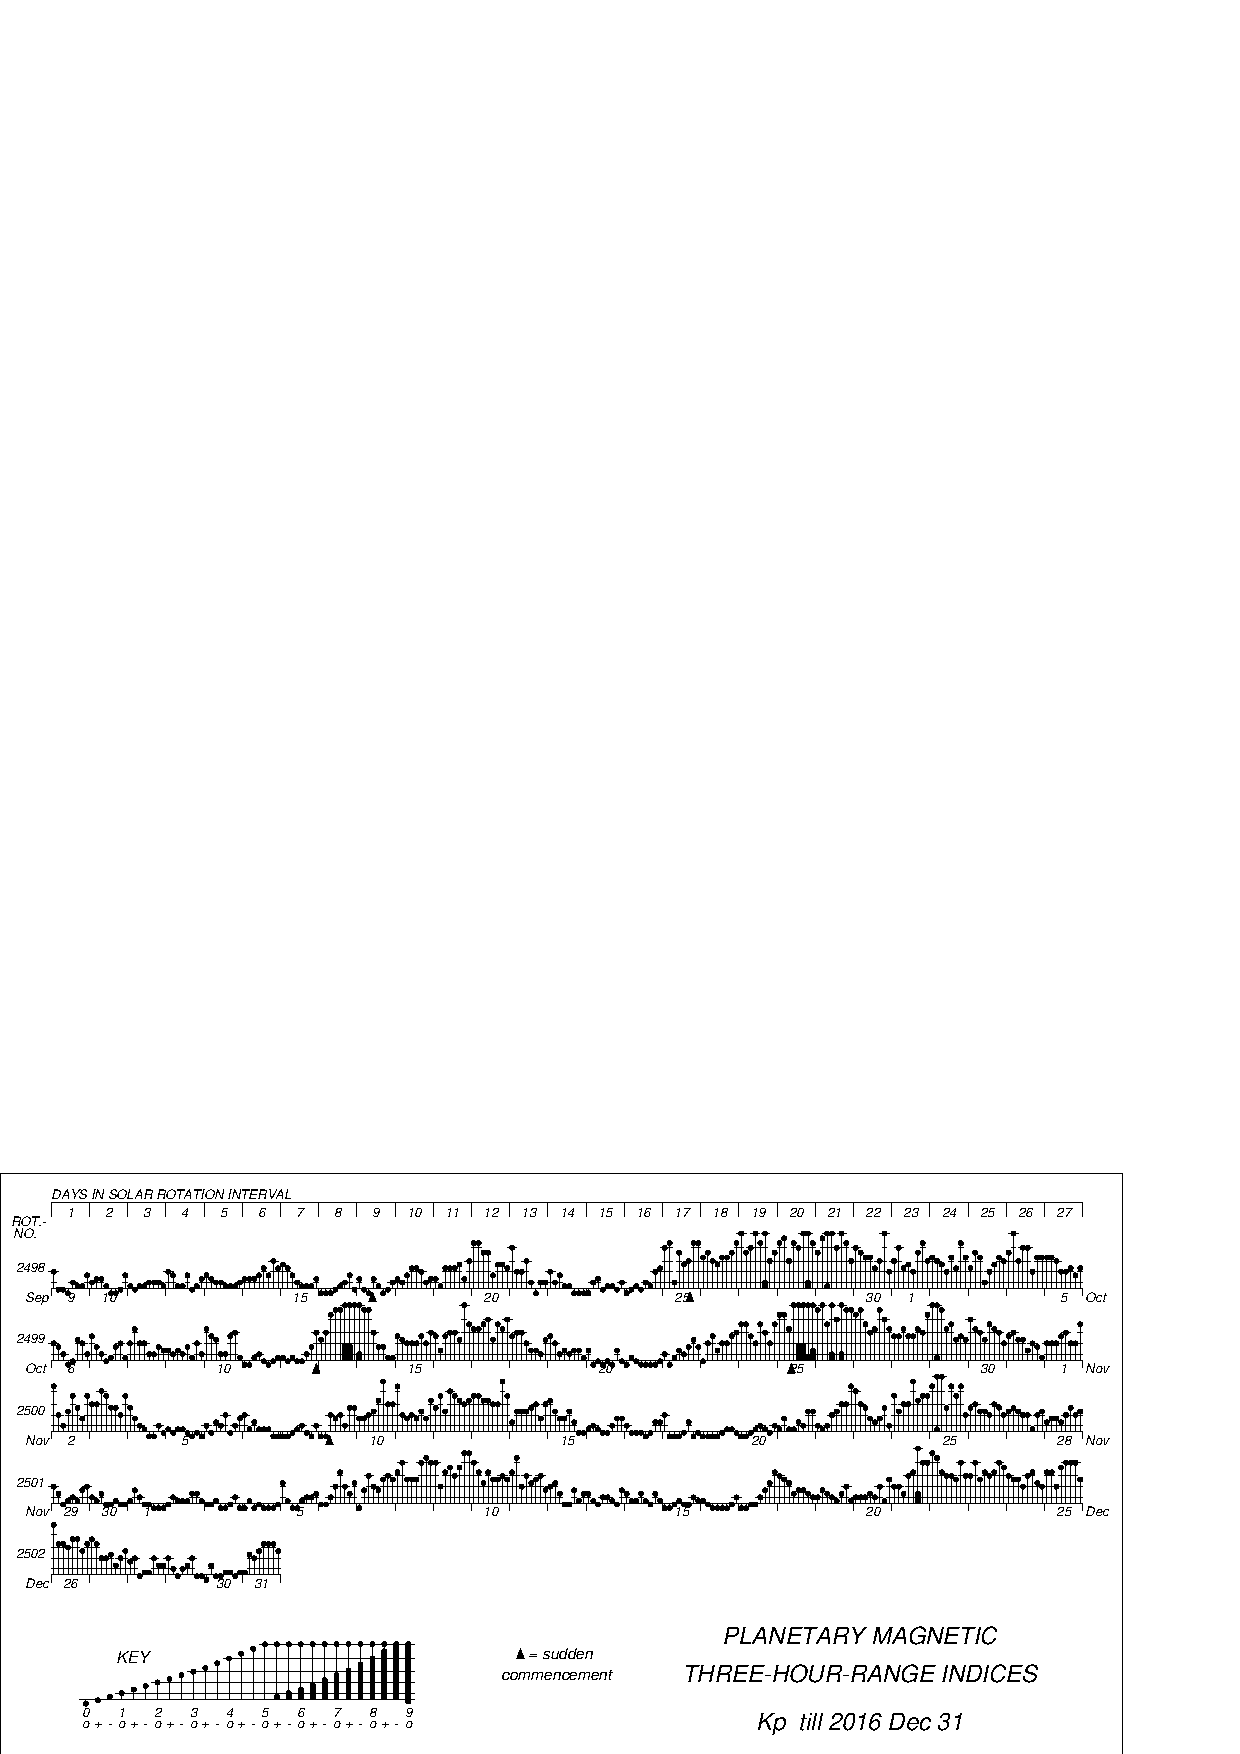
\includegraphics[width=\textwidth]{images/musi1612.pdf}
	\caption{Bartels musical \Kp{} diagram for the time period from September until end of December 2016. Two sudden commencements with following geomagnetic storms, having a maximal \Kp{} of $6+$, can be seen in October. Credit: \href{http://www.gfz-potsdam.de/en/kp-index/}{GFZ~Potsdam}, 2017, licensed under \href{https://creativecommons.org/licenses/by/4.0/}{CC BY 4.0}.}
	\label{fig:musi1612}
\end{figure}
%ftp://ftp.gfz-potsdam.de/pub/home/obs/kp-ap/music/

The \Kp{}~index can be converted to the 3"~hour equivalent $ap$~index, which represents the magnetic field strength at a surface position of about \SI{50}{\degree} dipole latitude. The conversion is done via a table defined by Bartels, in which the value of the \textit{ap}~index is scaled in units of \SI{2}{nT} (see \autoref{tab:kp_to_ap_table}).
\begin{table}
	\caption{Defined table for the conversion from the \Kp~index to the equivalent \textit{ap}~index, which represents the magnetic field strength in units of \SI{2}{nT}.}
	\label{tab:kp_to_ap_table}
	\centering
	\begin{tabular}{lssssssssssssss}
		\Kp	&0o	&0+	&1-	&1o	&1+	&2-	&2o	&2+	&3-	&3o	&3+	&4-	&4o	&4+\\
		\textit{ap}	&0	&2	&3	&4	&5	&6	&7	&9	&12	&15	&18	&22	&27	&32\\
		\hline
		\Kp	&5-	&5o	&5+	&6-	&6o	&6+	&7-	&7o	&7+	&8-	&8o	&8+	&9-	&9o\\
		\textit{ap}	&39	&48	&56	&67	&80	&94	&111	&132	&154	&179	&207	&236	&300	&400
	\end{tabular}
\end{table}
There are further geomagnetic indices which are derived from the \Kp{}~index. They include $Ap$, the daily $ap$ average, $Cp$, the daily $ap$ sum mapped via a defined table to the range \numrange{0}{2.5}, and $C9$, a mapping of $Cp$ via a defined table to the range \numrange{0}{9}. The definitions of Q"~days (quiet days) and D"~days (disturbed days) are also obtained from the \Kp{}~index.

The International Association of Geomagnetism and Aeronomy (IAGA) adopted the \Kp{}~index in 1954. The \Kp{}~index was maintained in Göttingen until January 1997 -- now the German Research Centre for Geosciences (GFZ) in Potsdam supplies the \Kp{}~index and thereof derived indices. The GFZ provides historical and quicklook data of the indices via their website\footnote{GFZ website for geomagnetic indices: \url{http://www.gfz-potsdam.de/de/kp-index/} (existent in 2017-10-29)}. The data was extended backwards and is available from 1932 onwards.\\

Several indicators/quantities are based on the \Kp{}~index:\\
The NOAA G-Scale for geomagnetic storms (G~1 to G~5) is based on the \Kp~index\footnote{NOAA Space Weather Scales website: \url{http://www.swpc.noaa.gov/noaa-scales-explanation} (existent in 2017-10-29)}.\\
The equatorward auroral boundary position correlates with the \Kp~index (cite?).\\
The variation of the total electron content (TEC) of the ionosphere correlates with the \Kp~index (cite?). The TEC has influence on global navigation satellite systems (GNSS). A part of their positional error scales directly with TEC (in extreme cases up to about \SI{30}{\m}).\\

"It is designed to measure solar particle radiation by its magnetic effects."\\

Because of the effects on sensitive technical systems, methods for \Kp{} forecasting are developed.\\
- Wing \Kp{} model (link)\\
- Potsdam quicklook data (link)\\
- Alexej \Kp{} correlation forecast model (link)\\
- In this work we derive relations for \Kp{} nowcast from in-situ solar-wind measurements and \Kp{} forecast from remote solar-wind stream/CME observations.\\

% acknowledgments:\\
% The results presented in this thesis rely on the \Kp{}~index, calculated and made available by the German Research Centre for Geosciences in Potsdam from data collected at magnetic observatories. We thank the involved national institutes, the INTERMAGNET network and ISGI (isgi.unistra.fr).\\


\subsection{OMNI data set}
\label{sec:omni_data_set}

see paper...\\

a data set merged from different sources\\
The OMNI data \citep{King2005} were obtained from the GSFC/SPDF OMNIWeb interface.\\

from spacecraft located near the Lagrange point L1 upstream of Earth\\
time-shifted to the bow shock of the magnetosphere\\

OMNI2 H0 MRG1HR (1963--201308)
Cite from CDAweb: Hourly near-Earth solar-wind magnetic field and plasma data, energetic proton fluxes (>~1 to >~60~MeV), and geomagnetic and solar activity indices.

NASA, Goddard Space Flight Center (GSFC), Space Physics Data Facility (SPDF): \url{http://spdf.gsfc.nasa.gov/}\\	%exintent in 2016-08-18
- Coordinated Data Analysis Web (CDAWeb): \url{http://cdaweb.gsfc.nasa.gov/}\\	%exintent in 2016-08-18
- OMNIWeb Plus: \url{http://omniweb.gsfc.nasa.gov/}\\	%exintent in 2016-08-18
%OMNIWeb Data Documentation: http://omniweb.gsfc.nasa.gov/html/ow_data.html

intercalibrated multi-spacecraft solar-wind data\\
Various spacecraft contribute to the interplanetary magnetic field (IMF) and solar-wind plasma OMNI data, as seen in \autoref{fig:timeline_OMNI_SC_IDs}.\\
\begin{figure}[htb]
	\centering
	\includegraphics[width=\textwidth]{images/gnuplots/timeline_OMNI_SC_IDs.pdf}
	\caption{IMF and solar-wind plasma data source spacecraft for the high and the low resolution OMNI (HRO, LRO) data sets until end of 2016. The SIDC 13-month smoothed monthly SSN is plotted in the background. add cycle number...}
	\label{fig:timeline_OMNI_SC_IDs}
\end{figure}

\subsubsection{Solar Wind Structures}
Solar Wind Structures (SWS) list\\
derived by Richardson.... from OMNI data (only?)
see chapter2...\\

permission received.\\

%http://cedarweb.vsp.ucar.edu/wiki/index.php/Tools_and_Models:Solar_Wind_Structures
characterization of near-Earth solar-wind structures since 1963\\
SWS lists \citep{Richardson2000} and \citep{Richardson2012}


\subsection{Helios probes}
\label{sec:helios_probes}

see Helios data readme.txt\\
see paper\\

two different fluxgate magnetometers and a search coil magnetometer\\

see \autoref{fig:helios2}
\begin{figure}[htb]
	\begin{floatrow}
		\ffigbox[\FBwidth][]{
			\includegraphics[width=0.3\textwidth]{images/helios2.jpg}
		}{
			\caption{One of the nearly identical twin Helios spacecraft. Credit: \href{https://solarsystem.nasa.gov/galleries/helios}{NASA/Max Planck Institute for Solar System Research}.}
			\label{fig:helios2}
			%source: https://solarsystem.nasa.gov/galleries/helios
			%NASA has no copyrights to its contents
		}
		\ffigbox[\Xhsize]{
			\includegraphics{images/gnuplots/Helios12_1h_r_b_ssn_plot.pdf}
		}{
			\caption{Plot of the Helios probes' solar distance and HGI latitude over their mission time, together with the monthly SSN and 13-month smoothed monthly SSN.}
			\label{fig:Helios12_1h_r_b_ssn_plot}
		}
	\end{floatrow}
\end{figure}

solar distance, HGI latitude and sunspot number during the Helios missions; see \autoref{fig:Helios12_1h_r_b_ssn_plot}\\

Helios~1 and 2 orbits in the ecliptic plane and in the latitude polar plane (see \autoref{fig:Helios12_orbits_ecliptic_polar})\\
\begin{figure}[htb]
	\centering
	\includegraphics[width=\textwidth]{images/gnuplots/Helios12_orbits_ecliptic_polar.pdf}
	\caption{Orbits of the Helios~1 (red) and Helios~2 (green) spacecraft in the solar equatorial plane (left) and polar plane (right) (HGI-coordinates). change colors?}
	\label{fig:Helios12_orbits_ecliptic_polar}
\end{figure}

The Helios magnetic field and plasma data frequency over heliocentric distance and over heliographic latitude are plotted in \autoref{fig:helios_data_frequency}.\\
\begin{figure}[htb]
	\centering
	\includegraphics[width=\textwidth]{images/gnuplots/helios_data_frequency.pdf}
	\caption{Helios data frequency over heliocentric distance with bins of \SI{0.01}{au} (left panels) and over heliographic latitude with bins of \SI{0.1}{\degree} (right panels). The frequency data is based on the hourly merged magnetometer and plasma data sets for Helios~1 and Helios~2. The top panels show the frequencies for Helios~1 and Helios~2 individually and the bottom panels those for the magnetometer and plasma data. avoid white lines...}
	\label{fig:helios_data_frequency}
\end{figure}

Solar wind data courtesy of R.~Schwenn, Max-Planck-Institut für Aeronomie, Lindau, magnetic field data courtesy of F.~Neubauer, Universität zu Köln. (see paper; into acknowledgements...)\\

%see presi 1.07 Inside Helios-Origins and Evolution-Salem.ppt
%see book Schwenn1990 https://books.google.de/books?id=W1DuCAAAQBAJ&printsec=frontcover&dq=Physics+of+the+Inner+Heliosphere+I.+Large-Scale+Phenomena&hl=de&sa=X&redir_esc=y#v=onepage&q=Physics%20of%20the%20Inner%20Heliosphere%20I.%20Large-Scale%20Phenomena&f=false



data sources -- see paper for replacing the following data\\
solar-wind parameters: ACE, Helios, OMNI\\
geomagnetic indices: Kp, OMNI\\

Space Physics Data Facility (SPDF)\\

HELIOS~1 and 2 - orbital Parameters\\
\url{http://spdf.sci.gsfc.nasa.gov/pub/data/helios/helios1/traj/}\\
\url{http://spdf.sci.gsfc.nasa.gov/pub/data/helios/helios2/traj/}\\

Helios hourly merged mag \& plasma data:\\
HELIOS1\_COHO1HR\_MERGED\_MAG\_PLASMA\_2965.txt\\
HELIOS2\_COHO1HR\_MERGED\_MAG\_PLASMA\_3096.txt\\
\url{http://cdaweb.gsfc.nasa.gov}\\
temporal coverage of merged data\\
Helios 1: 1974-12-10 - 1981-06-14\\
Mag data availability: 42.6~\%\\
Plasma \& orbit data availability: 76.4~\%\\
Helios 2: 1976-01-01 - 1980-03-04\\
Mag data availability: 54.4~\%\\
Plasma \& orbit data availability: 91.8~\%\\


\subsection{Real-time solar-wind data}

Advanced Composition Explorer (ACE)\\
s/c figure, launch date was 25 August 1997\\

Wind, STEREO, SOHO, CELIAS\\

data errors/gaps...\\
Several services/alerts are based on the data streams from real-time measurements. (L1 alerts, etc.)\\

DSCOVR as replacement was launched on 11~Februar 2015. It is NOAA's SWPC real-time solar-wind prime source since 27 July 2016.\footnote{\url{http://www.swpc.noaa.gov/products/real-time-solar-wind}}\\
		%introduction & basics
%	\chapter{Data}
\label{chap:data}

	\chapter{Solar wind time variations}
\section{Solar wind variation with solar cycle}
\section{Solar wind variation with season}
\section{Solar wind empirical forecast}

\chapter{Solar wind distance variations}
\section{Solar wind back-extrapolation}


%COFI -- chapter outline and flow integration\\

see paper...\\

McGregor2011 analyzed the empirical magnetic topology–velocity relationship, using Helios perihelion data with the Wang-Sheeley-Arge (WSA) coronal model, and found indications, that the fast and slow solar wind are generated from distinct sources. (not only superradial expansion)\\


	\chapter{Helios radial line-up passings}

%COFI -- chapter outline and flow integration\\

have a look into Schwenn1984...\\

%motivation
To derive the radial dependence of the solar wind parameters directly, we look at the passings when both Helios spacecraft were radially lined up. In these cases they flew through the same solar wind at different solar distances.\\
(This eliminates the bias of averaging over slow and fast wind streams, like the described model does.)\\
see also \citet{Schwenn1990} p.~156 + p.~122...\\
%Helios line-up mapping techniques -> Schwenn1981 "Two states..." (not findable online after extensive search)

we compare these independently derived radial fit functions to those obtained from the averaging over all solar wind types...\\

%Helios passings, their time and position
There were eight passings when both Helios spacecraft were radially lined-up (see \autoref{fig:Helios12_lineup_positions_v3_pdfcairo_plot}).
\begin{figure}[htb]
	\centering
	\includegraphics[width=0.6\textwidth]{images/gnuplots/Helios12_lineup_positions_v3_pdfcairo_plot.pdf}
	\caption{Schema of the eight spacecraft line-up positions of both Helios probes on their respective orbits. make B\&W... combine with fig 5.15? calibrate text size}
	\label{fig:Helios12_lineup_positions_v3_pdfcairo_plot}
\end{figure}
These points in time, when both probes had no separation in heliographic longitude, are derived from Helios~1 and Helios~2 daily trajectory data (for the data source see Section~XX). The data is linear interpolated to get an hourly resolution. The resulting points in time together with solar distances are listed in \autoref{tab:lineup_in_longitude}.
\begin{table}[htb]\small
	\centering
	\captionsetup{belowskip=4pt}
	\caption{Times when both Helios probes had no separation in heliographic longitude. Their solar distances (inner spacecraft $r_1$, outer spacecraft $r_2$) were in the range 0.291--0.731~au and the maximal inter-probe radial distance d$r$ was 0.229~au. errors in au...}
	\begin{tabular}{ccccccc}
		\toprule
		\multirow{2}{*}{Passing}	&\multirow{2}{*}{Date}	&\multirow{2}{*}{Time}	&\multirow{2}{*}{Inner s/c}	&$r_1$	&$r_2$	&d$r$\\
			&	&	&	&[au]	&[au]	&[au]\\
		\midrule
		1	&1976-03-09	&00:00	&Helios 1	&0.513	&0.731	&0.219\\
		2	&1976-05-02	&14:00	&Helios 2	&0.442	&0.671	&0.229\\
		3	&1976-09-19	&10:00	&Helios 1	&0.457	&0.637	&0.180\\
		4	&1976-10-31	&11:00	&Helios 2	&0.390	&0.576	&0.186\\
		5	&1977-04-02	&12:00	&Helios 1	&0.394	&0.519	&0.125\\
		6	&1977-04-30	&23:00	&Helios 2	&0.337	&0.465	&0.128\\
		7	&1977-10-18	&06:00	&Helios 1	&0.316	&0.345	&0.029\\
		8	&1977-10-25	&19:00	&Helios 2	&0.291	&0.327	&0.035\\
		\bottomrule
	\end{tabular}
	\label{tab:lineup_in_longitude}
\end{table}
%table data from
%file:///home/raid0/mvenzmer/Desktop/astro70/analyses/Helios12_1h_magswe/Helios12_1h_inline/lineup_periods_v3.txt

%excluding period 7 and 8
The last two passings were merely one week apart and the Helios probes flew almost without radial separation because Helios~2 overtook Helios~1 during its perihelion. As we want to analyze the same solar wind at different solar distances, we exclude the passings 7 and 8 from further analyses.\\


%defining line-up requirements
The passing longitude is not the same as the longitude where the solar wind is detected by both spacecraft consecutively. A passing occurs shortly before the points in time when both spacecraft observe the same solar wind. For the outer probe this point in time is shifted by the solar wind's travel time. The travel time depends on the solar wind's velocity and its distance traveled.\\


%calculation of the offset times
Based on the obtained spacecraft line-up time $t_0$ one can calculate the offset times $t_1$ and $t_2$ when the inner and outer spacecraft pass by the same solar wind (see \autoref{fig:Helios12_lineup_calculation_pdfcairo_plot}). At the solar wind line-up longitude the condition
\begin{align}
	t_2 = t_1 + t_\text{sw} \label{eq:lineup_condition}
\end{align}
holds. As the offset times depend on the solar wind travel time between the probes, we need knowledge of the solar wind velocity $v$ for their calculation: $t_\text{sw} = \text{d}r/v$, with the mean radial separation distance d$r$ between the probes.
\begin{figure}[htb]
	\centering
	\includegraphics[width=0.5\textwidth]{images/gnuplots/Helios12_lineup_calculation_pdfcairo_plot.pdf}
	\caption{Illustration of the solar wind line-up longitude situation with the spacecraft line-up time $t_0$, the offset times $t_1$, $t_2$ (at which the spacecraft measure the same solar wind) and the solar wind travel time $t_\text{sw}$. combine with fig 5.14?}
	\label{fig:Helios12_lineup_calculation_pdfcairo_plot}
\end{figure}
%/home/raid0/mvenzmer/Desktop/astro70/analyses/Helios12_1h_magswe/Helios12_1h_inline/Helios12_lineup_calculation_pdfcairo_gps.txt

%calculating t_1
For the calculation of $t_1$ we recall the third Kepler law
\begin{align}
	\frac{{T_1}^2}{{T_2}^2} = \frac{{a_1}^3}{{a_2}^3}
\end{align}
with the orbital periods $T_1$, $T_2$ and the semi-major axes $a_1$, $a_2$. The assumption of circular orbits (why? what error size?) leads to
\begin{align}
	\frac{{t_1}^2}{(t_1 + t_\text{sw})^2} &= \frac{{r_1}^3}{{r_2}^3}	\nonumber\\
	\Leftrightarrow\qquad\qquad	t_1 &= t_\text{sw} \left( \left( \frac{r_1}{r_2} \right)^\frac{3}{2} - 1 \right)^{-1} \label{eq:offset_time}
\end{align}
and finally the offset time $t_1$ only depends on the variable solar wind travel time $t_\text{sw}$.\\

%calculating the offset time from the solar wind velocity
Due to uncertainties in the travel time $t_\text{sw}$ (the solar wind speed $v$ is obviously not a constant) the exact calculation of $t_1$ is imprecise. To get a reliable result we perform two iterations calculating the offset time from the average velocity $\bar{v}$ of the surrounding 2-day period. We use the velocity $\bar{v}_0$ around $t_0$ to calculate the offset time $t'_1$ as a first estimate. As the velocity $\bar{v}'_1$ at $t'_1$ is certainly different, we use this velocity to refine the value and obtain $t_1$. Hence deriving the velocity $\bar{v}_1$ enables us to calculate the solar wind travel time $t_\text{sw}$.

%We have to round the offset times and time shift values to full hours, because we use the hourly merged mag and plasma Helios data set (see Section~XX) for the velocity calculation.
The average velocities are obtained from the hourly merged (mag?) and (plasma?) Helios data set (see Section~XX). The resulting offset times and velocities of both iterations together with the travel times are listed in \autoref{tab:offset_times}.
\begin{table}[htb]\small
	\centering
	\captionsetup{belowskip=4pt}
	\caption{The two iterations of the derived offset times and average velocities. The resulting solar wind travel times have durations of 11--28~hours. errors...}
	\begin{tabular}{cccccccc}
		\toprule
		\multirow{2}{*}{Passing}	&\multirow{2}{*}{Inner s/c}	&$v_0$	&$t'_1$	&$v'_1$	&$t_1$	&$v_1$	&$t_\text{sw}$\\
			&	&[km/s]	&[h]	&[km/s]	&[h]	&[km/s]	&[h]\\
		\midrule
		1	&Helios 1	&659.3	&19.6	&656.9	&19.7	&656.9	&13.9\\
		2	&Helios 2	&436.4	&25.1	&370.9	&29.5	&356.7	&26.7\\
		3	&Helios 1	&482.6	&24.0	&444.0	&26.1	&413.8	&18.1\\
		4	&Helios 2	&302.3	&32.2	&279.9	&34.8	&278.3	&27.8\\
		5	&Helios 1	&507.3	&20.0	&474.8	&21.4	&473.5	&11.0\\
		6	&Helios 2	&321.2	&26.6	&392.6	&21.7	&367.8	&14.5\\
		\bottomrule
	\end{tabular}
	\label{tab:offset_times}
\end{table}
%table data from
%file:///home/raid0/mvenzmer/Desktop/astro70/analyses/Helios12_1h_magswe/Helios12_1h_inline/lineup_periods_v3.txt

%introducing the lag time for arbitrary longitude positions
For the solar wind line-up longitude condition~\eqref{eq:lineup_condition} holds. For all other positions the solar wind measured by the inner spacecraft will not arrive the outer orbit position at the same time as the outer spacecraft does (see \autoref{fig:Helios12_lineup_calculation_delay_pdfcairo_plot}).
\begin{figure}[htb]
	\centering
	\includegraphics[width=0.5\textwidth]{images/gnuplots/Helios12_lineup_calculation_delay_pdfcairo_plot.pdf}
	\caption{Illustration like \autoref{fig:Helios12_lineup_calculation_pdfcairo_plot} but for arbitrary longitude situations a lag time $t_\text{lag}$ comes into play. merge with fig 5.14?}
	\label{fig:Helios12_lineup_calculation_delay_pdfcairo_plot}
\end{figure}
%/home/raid0/mvenzmer/Desktop/astro70/analyses/Helios12_1h_magswe/Helios12_1h_inline/Helios12_lineup_calculation_delay_pdfcairo_gps.txt

Either the spacecraft (negative lag time) or the solar wind (positive lag time) already have passed this position:
\begin{align}
	t_2 = t_1 + t_\text{sw} + t_\text{lag}. \label{eq:lag_time}
\end{align}
This lag time $t_\text{lag}$ is the time difference at which the solar wind is probed by both spacecraft. At the spacecraft line-up longitude ($t_1 = t_2 = 0$) the lag time equals the solar wind travel time and at the solar wind line-up longitude the lag time is zero.\\

%calculation of the +-24 hour solar wind time span
We choose to look at time periods (instead of points in time) around the offset times to derive average solar wind parameters. This helps reducing the influence of solar wind fluctuations.\\

We define the period duration boundaries as when the lag time $t_\text{lag}$ is in the range $\pm24$~h. For the outer spacecraft these periods are almost twice as long as for the inner spacecraft. The calculated period start and end hours (relative to $t_0$) for both spacecraft are listed in \autoref{tab:period_times_coverage} together with the data coverage of these periods.
\begin{table}[htb]\small
	\centering
	\captionsetup{belowskip=4pt}
	\caption{Derived period start and end hours for both spacecraft in relation to the longitude line-up time $t_0$. The corresponding combined data coverage within that period of the magnetic field, velocity, density and temperature is listed as well. instead duration! errors...}
	\begin{tabular}{cccrrccrrc}
		\toprule
		\multirow{3}{*}{Period}	&	&\multicolumn{4}{c}{Inner spacecraft}	&	&\multicolumn{3}{c}{Outer spacecraft}\\
		\cmidrule{3-6}	\cmidrule{8-10}
			&	&\multirow{2}{*}{s/c}	&Start	&End	&Coverage	&	&Start	&End	&Coverage\\
			&	&	&[h]	&[h]	&[\%]	&	&[h]	&[h]	&[\%]\\
		\midrule
		1	&	&Helios 1	&-14.4	&53.8	&73	&	&-24.6	&91.6	&99\\
		2	&	&Helios 2	&3.1	&58.3	&89	&	&5.8	&109.0	&88\\
		3	&	&Helios 1	&-9.2	&65.1	&16	&	&-15.1	&107.2	&10\\
		4	&	&Helios 2	&4.8	&65.2	&59	&	&8.5	&117.0	&87\\
		5	&	&Helios 1	&-25.5	&68.3	&89	&	&-38.5	&103.3	&88\\
		6	&	&Helios 2	&-15.3	&61.7	&93	&	&-24.8	&100.1	&92\\
		\bottomrule
	\end{tabular}
	\label{tab:period_times_coverage}
\end{table}
% %table data from
% %file:///home/raid0/mvenzmer/Desktop/astro70/analyses/Helios12_1h_magswe/Helios12_1h_inline/lineup_periods_v3.txt

%excluding period 3
For period~3 the combined data coverage of the four solar wind parameters is only 16~\% (Helios~1) and 10~\% (Helios~2) respectively. We consider this as insufficient for the continuing analysis and therefore also omit period~3.\\

The five remaining periods are marked in \autoref{fig:Helios12_lineup_period_positions_v3_pdfcairo_plot}.
\begin{figure}[htb]
	\centering
	\includegraphics[width=0.6\textwidth]{images/gnuplots/Helios12_lineup_period_positions_v3_pdfcairo_plot.pdf}
	\caption{Scheme of the line-up periods of both Helios spacecraft on their respective orbits. The corresponding orbit sections which we consider in our analysis are marked in color. These sections span the positions where both spacecraft observed the same solar wind with a maximal lag time of $\pm24$~hours. bw figure?? dotted lines?}
	\label{fig:Helios12_lineup_period_positions_v3_pdfcairo_plot}
\end{figure}

%average values
The average values of the four parameters magnetic field $B$, velocity $v$, density $n$ and temperature $T$ are listed in \autoref{tab:period_means}.
\begin{table}[htb]\small
	\centering
	\captionsetup{belowskip=4pt}
	\caption{Average values of the four solar wind parameters magnetic field, velocity, density and temperature for the individual periods and spacecraft. errors...}
	\begin{tabular}{cccrrrrcrrrr}
		\toprule
		\multirow{3}{*}{Period}	&	&\multicolumn{5}{c}{Inner spacecraft}	&	&\multicolumn{4}{c}{Outer spacecraft}\\
		\cmidrule{3-7}	\cmidrule{9-12}
			&	&\multirow{2}{*}{s/c}	&\multicolumn{1}{c}{$B$}	&\multicolumn{1}{c}{$v$}	&\multicolumn{1}{c}{$n$}	&\multicolumn{1}{c}{$T$}	&	&$B$	&$v$	&$n$	&$T$\\
			&	&	&\multicolumn{1}{c}{[nT]}	&\multicolumn{1}{c}{[km/s]}	&\multicolumn{1}{c}{[cm$^{-3}$]}	&\multicolumn{1}{c}{[K]}	&	&[nT]	&[km/s]	&[cm$^{-3}$]	&[K]\\
		\midrule
		1	&	&Helios 1	&17.04	&646.4	&12.0	&367\,300	&	&8.93	&602.8	&6.7	&244\,000\\
		2	&	&Helios 2	&15.77	&356.4	&38.8	&122\,400	&	&12.05	&390.2	&17.7	&117\,200\\
		4	&	&Helios 2	&15.18	&281.3	&108.0	&46\,000	&	&10.64	&298.6	&46.1	&30\,400\\
		5	&	&Helios 1	&28.80	&521.3	&45.9	&337\,800	&	&18.73	&530.3	&24.4	&282\,000\\
		6	&	&Helios 2	&29.57	&402.4	&82.5	&271\,900	&	&14.71	&432.6	&35.7	&199\,100\\
		\bottomrule
	\end{tabular}
	\label{tab:period_means}
\end{table}
%table data from
%file:///home/raid0/mvenzmer/Desktop/astro70/analyses/Helios12_1h_magswe/Helios12_1h_inline/lineup_periods_v3.txt

%solar wind feature match
If we compare both, the inner solar wind sections together with their outer counterparts, they indeed appear to have a similar shape apart from the time shift (see \autoref{fig:Helios12_lineup_period_1_7d_v3_plot}) (name definite features...). This confirmes that they indeed are parts of the same solar wind structures.\\
maybe figures of all into Appendix?...\\
\begin{figure}[htb]
	\centering
	\includegraphics[width=0.5\textwidth]{images/gnuplots/Helios12_lineup_period_1_7d_v3_plot.png}
	\caption{Measured solar wind parameters $B$, $v$, $n$, and $T$ of both spacecraft in the period~1. Also plotted is the spacecraft's separation in heliographic longitude. offset time, time shift; expected value from the radial sw model... remove date... remove solar distance... adjust text size...}
	\label{fig:Helios12_lineup_period_1_7d_v3_plot}
\end{figure}


%solar wind types
the comparison to the sw model's mean value at the individual distances lets us classify the solar wind types...
\begin{description*}
	\item[Period 1]	HSS
	\item[Period 2]	medium--LSS
	\item[Period 4]	LSS
	\item[Period 5]	medium--HSS
	\item[Period 6]	LSS--HSS
\end{description*}

%...forward- and back-matching data gaps results in worse data coverage!

%fit function parameters
We obtained the mean parameter values for the inner and outer solar wind sections. As with the overall radial dependency before, these two points are fitted to the exponential regression fit function $X(r) = X_0\,r^{c_X}$ (see Section~XX. The resulting fit coefficients for each period are listed in \autoref{tab:lineup_fit_functions}.\\
why is it better to fit the period's mean values than the whole period?...\\
we fit the periods' mean value rather than the whole periods, because...\\

\begin{table}[htb]\small
	\centering
	\captionsetup{belowskip=4pt}
	\caption{Radial fit functions $B(r)$, $v(r)$, $n(r)$ and $T(r)$ for each period. or only the variables into table? error sizes...}
	\begin{tabular}{cgggg}
		\toprule
		\multirow{2}{*}{Period}	&B(r) =,B_0~r^{c_B}	&v(r) =,v_0~r^{c_v}	&n(r) =,n_0~r^{c_n}	&T(r) =,T_0~r^{c_T}\\
			&\text{[nT]},	&\text{[km/s]},	&\text{[cm$^{-3}$]},	&\text{[K]},\\
		\midrule
		1	&4.88,r^{-1.815}	&564.7,r^{-0.196}	&3.9,r^{-1.647}	&166\,500,r^{-1.148}\\
		2	&9.50,r^{-0.654}	&442.6,r^{0.220}	&8.9,r^{-1.902}	&112\,800,r^{-0.106}\\
		4	&6.79,r^{-0.900}	&322.0,r^{0.151}	&15.7,r^{-2.155}	&18\,000,r^{-1.047}\\
		5	&5.99,r^{-1.649}	&554.8,r^{0.065}	&4.6,r^{-2.423}	&174\,700,r^{-0.692}\\
		6	&3.22,r^{-2.108}	&506.5,r^{0.219}	&5.7,r^{-2.533}	&101\,000,r^{-0.941}\\
		\midrule
		weigthed by duration mean functions\\
		\midrule
		mean of sw model (update)	&6.078,r^{-1.563}	&435.5,r^{0.04955}	&7.613,r^{-2.032}	&97\,050,r^{-0.8002}\\
		\bottomrule
	\end{tabular}
	\label{tab:lineup_fit_functions}
\end{table}
%table data from
%file:///home/raid0/mvenzmer/Desktop/astro70/analyses/Helios12_1h_magswe/Helios12_1h_inline/lineup_periods_v3.txt

%interpretation
The fit curves show noticeable deviations from the model's mean fit (see \autoref{fig:Helios12_lineup_fit_Bmean_v3_final_plot}). maybe 4-panel figure?; maybe figures of all into Appendix?\\
\begin{figure}[htb]
	\centering
	\includegraphics[width=0.5\textwidth]{images/gnuplots/Helios12_lineup_fit_Bmean_v3_final_plot.png}
	\caption{Fit curves of the radial magnetic field. The fits are based on the mean values (meanr,meanB; black points) of the line-up periods. build pdf figure... remove date... adjust text size... 4-figure?}
	\label{fig:Helios12_lineup_fit_Bmean_v3_final_plot}
\end{figure}
The observed deviations are as expected from these types of solar wind. ...are they? analyze each in detail...\\
argue from sw type; slow, medium and fast type; check their position relative to the mean curve...\\

%what we have learned
results:\\
features of calculated line-up periods match.\\
their derived fit functions scatter within (acceptable?) margin around model's radial mean, backing its applicability.\\



	
\chapter{notes to chapter2...}

% Alle Presis ausschlachten!\\
% Alle Projektberichte ausschlachten!\\
% Kp8--Liste irgendwo einweben...\\

-> example events CIR/HSS and CME\\

%the relation of these events was confirmed two decades ago by (who and \citet{Bothmer1993})\\


\section{Solar wind structure analyses}
How strong do different structure types influence the terrestrial magnetosphere?\\
What kind of solar wind structures create the individual regions in this distribution?\\
What is their individual contribution to the Kp ranges (e.g. high Kp: CMEs 70\% and CIRs 30\%)?\\

ACE solar wind time series and event list\\
sw-timeseries ACE OPTIMAP ``Zeitreihe''-events

method: automatic list creation by event detection via parameter thresholds...\\

sample CME analyses (MVA -> Kp)\\


\section{Forecast}
How can the impact field strength of CMEs be forecasted (V->B correlation for CMEs)?\\
Internal solar wind correlations:\\
B-V correlation\\
ACE MAGSWE 64~s data -> yearly overlay plot\\

applications:\\
rssfeeds, rtsw plots\\
CME Kp impact as part of DDC\\
- \textit{Kp} nowcast with L1 solar wind measurements (L1 alerts, disseminated as RSS feeds; integrated in smartphone app and space weather display)\\
- Forecast of the possible CME impact on the Earth's magnetosphere (\textit{Kp} index) from the predicted CME arrival velocity (integrated in UGOE CME forecast chain (aka DDC))\\


	
\chapter{Solar wind impact on the terrestrial magnetosphere}

% Alle Presis ausschlachten!
% Alle Projektberichte ausschlachten!
% Kp8--Liste irgendwo einweben...
% paper draft 2014 ausschlachten... Check!

%Questions addressed in this thesis
Questions:\\
	How strong is the solar wind influence on the terrestrial magnetosphere?\\
	How strong do different structure types influence the terrestrial magnetosphere?\\
	
	How can the impact strength of the solar wind be forecasted? (VBz->Kp L1-Alerts)\\
	How can the impact strength of CMEs be forecasted (V->Kp correlation for CMEs)?\\
	(How can the impact field strength of CMEs be forecasted (V->B correlation for CMEs)?)\\

On solar wind acceleration and SPP proposition: McComas2007\\

% Analyses structure:\\
% 
% Core studies:
% Motivational question: Which solar wind structures contribute to the individual Kp ranges?
% define OMNI data set duration
% build Kp histogram
% 	for each Kp range
% 		extract contributing solar wind sections
% 			get sections structure flag
% 		derive individual structure contribution
% 
% preparations:
% analyze solar wind and categorize its structure types
% 	define thresholds for event recognition
% 	write automatic event recognition program
% 	=> flagged time series
% 	(additional output: OMNI solar wind event list)
% 
% applications:
% - Kp nowcast with L1 solar wind measurements (L1 alerts, disseminated as RSS feeds; integrated in smartphone app and space weather display)
% - Forecast of the possible CME impact on the Earths magnetosphere (Kp index) from the predicted CME arrival velocity (integrated in UGOE CME forecast chain (aka DDC))
% 
% 
% Further studies:
% Motivational question: What is the evolution of the solar wind parameters/structures before arriving at Earth? %what is meant by the term evolution?
% define Helios data set
% extrapolation of the solar wind parameters with the use of regression fitting
% extraction of distance independent time series with regression fits
% get flagged time series from distance independent time series
% (like before:)
% analyze solar wind and categorize its structure types
% 	define thresholds for event recognition
% 	write automatic event recognition program
% 	=> flagged time series
% 	(additional output: Helios solar wind event list)
% 
% 
% empirical radial solar wind model:
% derive the characteristic distributions of the solar wind parameters from OMNI data
% combination of the OMNI characteristic distributions with the Helios extrapolation
% 	(additional output: empirical radial probability distribution model)
% 
% Applications:
% - The near-sun* solar wind extrapolation can be useful for the planned Solar Probe Plus mission


\section{Quantifying solar wind impact on the terrestrial magnetosphere}

linear velocity replacement of ACE realtime data with Kp, Machol2013\\

3hmin(vBzgsm) performs in rank correlation slightly better than the sophisticated Newell formula\\

choosing solar wind parameters\\
	comparison of their correlation coefficients in table...\\
		-> Pearson or Spearman rank cc?? (Appendix?)\\
		-> lag meaning?\\
	% bulk correlation coefficients and functions\\
	% B-Kp, V-Kp, Bz-Kp
	
What kind of correlation function with these parameters?\\
% comparison with existing solar wind-magnetosphere coupling functions (see Basics chapter)\\

comparison of correlation coefficients for different data resolutions and measures in \autoref{tab:cc_measure_comparison}.
\begin{table}[htb]\small
	\centering
	\captionsetup{belowskip=4pt}
	\caption{Pearson correlation coefficients of Kp with sample solar wind parameters for different data resolutions and measures for comparison. 3h 1min extrema data results in slightly higher ccs... (use Spearman instead?)}
	\begin{tabular}{lcccc}
		\toprule
			&OMNI 1h	&OMNI 1h	&OMNI 1min	&OMNI 1min\\
			&1963-201308	&1963-201308	&19850101-20150101	&19850101-20150101\\
			&3h mean	&3h 1h extrema	&3h 10min extrema	&3h 1min extrema\\
		\midrule
		V	&0.568	&0.579	&?	&0.598\\
		B	&	&	&	&\\
		\bottomrule
	\end{tabular}
	\label{tab:cc_measure_comparison}
\end{table}


correlation coefficients in \autoref{tab:correlation_coefficients}.
\begin{table}[htb]\small
	\centering
	\captionsetup{belowskip=4pt}
	\caption{Pearson correlation coefficients of Kp with solar wind parameters... (use Spearman instead?)}
	\begin{tabular}{cc}
		\toprule
			&OMNI 1min\\
		Parameter	&19850101-20150101\\
			&3h 1min max\\
		\midrule
		N	&0.199792\\
		V	&0.598351\\
		T	&0.510607\\
		B	&0.595860\\
		Bzgsm	&-0.666050$^\text{a}$\\
		V*B	&0.682383\\
		V*Bzgsm	&-0.715101$^\text{a}$\\
		N*T	&\\
		\bottomrule
		\multicolumn{2}{l}{\footnotesize{$^\text{a}$Here it is min instead of max.}}
	\end{tabular}
	\label{tab:correlation_coefficients}
\end{table}


Results of this section\\
What kind of solar wind structures create the individual regions in this distribution? -> next section\\
What is their individual contribution to the Kp ranges (e.g. high Kp: CMEs 70\% and CIRs 30\%)? -> next section\\

maybe correlation coefficient frequency spectra over time...?\\


\section{Solar wind structure type influence on the terrestrial magnetosphere}

Kp vs VBzgsm - CMEs as fraction of overall solar wind; see \autoref{fig:OMNI_HRO_1MIN_19810101-20130731_with_ap_vBzgsm_3hmin_CMEpart_VBzgsmvsKp_2Dhistogram_plot}
\begin{figure}[htb]
	\centering
	\includegraphics[width=0.3\textwidth]{images/gnuplots/OMNI_HRO_1MIN_19810101-20130731_with_ap_vBzgsm_3hmin_CMEpart_VBzgsmvsKp_2Dhistogram_plot.png}
	\caption{CMEs as fraction of overall solar wind. sws1/sws}
	\label{fig:OMNI_HRO_1MIN_19810101-20130731_with_ap_vBzgsm_3hmin_CMEpart_VBzgsmvsKp_2Dhistogram_plot}
\end{figure}

\subsection{Solar wind seasonal dependence}
seasonal variation by month\\
quantify variation amplitudes\\

see \autoref{fig:OMNI_monthly_freq_V_gps}
\begin{figure}[htb]
	\centering
	\includegraphics[width=0.3\textwidth]{images/gnuplots/OMNI_monthly_freq_V_gps.png}
	\caption{Diagram of the velocity frequency by month for the period 1963/01--2013/08. Mean and median values are shown as well.}
	\label{fig:OMNI_monthly_freq_V_gps}
\end{figure}

derived exponent values from simple trigonometric fit on monthly values:\\
$c_N = -2.234$\\
maybe figure?\\

...following maybe into section 'radial dependence of median value?\\
expected influence from perihelion/aphelion (see Appendix...) distance vs observations\\
we expect for the proton density (scaling law $N(r) = 7.6~\text{cm}^{-3} \cdot r^{-2}$):\\
N(0.983~au) = 7.9~cm$^{-3}$\\
N(1~au) = 7.6~cm$^{-3}$\\
N(1.017~au) = 7.3~cm$^{-3}$\\
we expect for the magnetic field strength (scaling law $\propto r^{-1.6}$):\\
B(0.983~au) = 6.3~nT\\
B(1~au) = 6.1~nT\\
B(1.017~au) = 5.9~nT\\

see \autoref{fig:OMNI_monthly_freq_B_a_gps}
\begin{figure}[htb]
	\centering
	\includegraphics[width=0.3\textwidth]{images/gnuplots/OMNI_monthly_freq_B_a_gps.png}
	\caption{Diagram of magnetic field frequency by month for the period 1963/01--2013/08. Mean and median values are shown as well as the expected course from the solar distance variation (obtained from Helios data).}
	\label{fig:OMNI_monthly_freq_B_a_gps}
\end{figure}

\section{Kp solar cycle dependence}
- solar cycle variations\\
- variations between solar cycles\\

the yearly Kp frequency shows variations; the yearly mean Kp shifts about 2~units.\\
plot of the yearly Kp frequency (see \autoref{fig:Kp_freq_yearly_ssn_plot})
\begin{figure}[htb]
	\centering
	\includegraphics[width=0.3\textwidth]{images/gnuplots/Kp_freq_yearly_ssn_plot.png}
	\caption{Kp frequency by year, yearly mean Kp and yearly mean total SSN for the years 1932--2015. The pattern of Kp shows an imprint of the solar cycle. Kp data from GFZ German Research Centre for Geosciences, Potsdam, Germany and SSN data from WDC-SILSO, Royal Observatory of Belgium, Brussels.}
	\label{fig:Kp_freq_yearly_ssn_plot}
\end{figure}
add Kp--SSN matrix plot...\\

analyze Kp frequency by month for different SWSs\\
analyze Kp frequency by year for different SWSs\\
put into later part of analysis...

\subsection{Kp seasonal dependence}
for high Kp values (>~4?) there are yearly frequency maxima at the equinoxes and minima at the solstices. this variation amounts to more than 1~Kp (see figure...)

possible causes (see \citet{Rangarajan1997} p. 1282 and mention Bartels1963 too):\\
- Earth's rotation axis tilt ($\pm23.44$\textdegree) (obliquity to orbit/inclination of equator)\\
- solar rotation axis tilt ($\pm7.25$\textdegree) (cite 'NASA Earth fact sheet')\\
- varying distance from Sun 0.983--1.0167~au ($\pm3.3~\%$)\\
- changing solar cycle polarity gives two superimposed maxima... -> No. see even/odd plots\\

read Bothmer1998 Ch 3...\\


\section{Summary/Results}
sw-nowcast: vBzgsm-Kp relation (average and worst case)\\
CME-forecast: v-Kp relation (average and worst case)\\

seasonal correction: $\Delta$Kp(month)\\
$Kp_\text{impact} = Kp_\text{CME} \pm \Delta Kp(month)$\\

sw-timeseries ACE OPTIMAP ``Zeitreihe''-events

\section{Forecast}

\subsection{Internal solar wind correlations}
B-V correlation\\
ACE MAGSWE 64~s data -> yearly overlay plot\\

\section{Applications}
rssfeeds, rtsw plots\\
CME Kp impact\\
part of DDC\\


	\chapter[Discussion and results]{Discussion/conclusions/results}
%\label{chap:}

%COFI -- chapter outline and flow integration\\

discussion\\
conclusions\\
results\\

Prediction:\\
Link from near-Sun solar wind measurements to Kp impact\\
Link from near-Sun structure (CMEs, CIRs) measurements to Kp impact\\

	\include{chapters/summary}	%summary and conclusions

	\appendix
	
\chapter{Physics}
\label{chap:physics}

\section{Electromagnetism}	%maybe exclude this section?

Electromagnetism is one of the four fundamental forces at the common level of energy. In all situations examined in this thesis (sw plasma, magnetosphere) it is by far the strongest force and the others can be neglected.\\

%Lorentz force law as the definition of E and B\\
%The electromagnetic force F on a test charge at a given point and time is a certain function of its charge q and velocity v, which can be parameterized by exactly two vectors E and B, in the functional form: (wiki)\\
The Lorentz force: $\textbf{F} = q (\textbf{E} + \textbf{v} \times \textbf{B})$\\

The Maxwell equations in differential notation:
\begin{align}
	\text{div}\,\textbf{B} &= 0\\
	\text{div}\,\textbf{D} &= \rho\\
	\text{rot}\,\textbf{H} &= \textbf{j} + \dot{\textbf{D}}\\
	\text{rot}\,\textbf{E} &= - \dot{\textbf{B}}
\end{align}
With the magnetic flux density \textbf{B} (aka magnetic field), the electric displacement field \textbf{D}, the charge density $\rho$, the magnetic field \textbf{H}, the electric field \textbf{E} and the current density \textbf{j}.\\
%note about B naming convention within this work as magnetic field strength% maybe put into beginning...


\section{Solar wind pressures}

The magnetic energy density $w_\text{mag}$ is also the magnetic pressure $p_\text{mag}$
\begin{align}
	w_\text{mag} &= p_\text{mag}\\
	&= \frac{B^2}{2 \mu_0}	\text{\,.}
\end{align}

dynamic pressure $p_\text{dyn} = \rho v^2$\\
thermal pressure $p_\text{therm} = n k_\text{B} T$\\
magnetic pressure $p_\text{mag} = B^2 / (2 \mu_0)$ (see above...)\\
ram pressure??\\
%VB1998p104


\section{Plasma beta}
\label{sec:plasma_beta}
In MHD the magnetic energy density behaves like an additional pressure that adds to the gas pressure of a plasma (Wikipedia; find alternative source...).

The ratio of the thermal pressure $p = n k_\text{B} T$ to the magnetic pressure $p_\text{mag} = \frac{B^2}{2 \mu_0}$ is called plasma beta
\begin{align}
	\beta &= \frac{p}{p_\text{mag}}\\
	&= \frac{2 \mu_0 n k_\text{B} T}{B^2}
\end{align}
with the number density $n$.\\
$\beta \ll 1$: ``cold'' plasma; magnetic field contains plasma (magnetic clouds)\\
$\beta \geq 1$: ``warm'' plasma; plasma keeps magnetic field

%aka proton beta
plasma beta see \citep[p.~50]{Kivelson1995}

typical $beta$-values for solar wind are in the range X--Y.\\

% Plasma beta:\\
% near-sun β << 1:\\
% far-sun β ≥ 1:\\
% β = p /pkin mag\\
% plasma follows magnetic field\\
% magnetic field is frozen within plasma\\
% --> spiral-like B-field\\
% Bφ ≈ -45° @ 1 au\\


\section{Alfvén waves}	%Alfvén velocity
\label{sec:alfvén_waves}
%maybe MHD waves

named after Hannes~Alfvén...

There exists an incompressible wave mode which is a result of bending magnetic field lines called shear Alfvén wave.

In an ideal incompressible MHD plasma (viscosity $\mu = 0$ and electrical conductivity $\sigma = \infty$) the kinetic and magnetic energy density are of equal value: 
\begin{align}
	w_\text{kin} &= w_\text{mag}\\
	\frac{\rho v^2}{2} &= \frac{B^2}{2 \mu_0}	\nonumber
\end{align}
with the permeability constant
\begin{align}
	\mu_0 &= 4 \pi \cdot \SI{e-7}{\newton\per\ampere\squared}	\nonumber
	%&\approx \SI{1.25663e-6}{\newton\per\ampere\squared}
\end{align}
and the total mass density $\rho$ of the charged plasma particles.

So waves propagate with the so-called Alfvén velocity
\begin{align}
	v_\text{A} = \frac{|B|}{\sqrt{\mu_0 \rho}}	\text{\,.}
\end{align}
Their phase velocity is
\begin{align}
	v_\text{ph} = v_\text{A} \cos(\theta)
\end{align}
with $\theta$ the angle between wave propagation direction (k) and magnetic field line (B). => Alfvén waves travel along magnetic field lines. Alfvén waves are characterized by periodic disturbances in the magnetic field perpendicular to its direction, in the electric field, in the plasma velocity and in the current density. They do not affect the plasma density, plasma pressure and magnetic field magnitude.

Additionally, there exist two types of compressional waves within MHD plasmas, the fast-mode wave and the slow-mode wave. The phase speeds of the three MHD waves meet $v_\text{fast} \geq v_\text{A} \geq v_\text{slow}$. %block copy from Kivelson1995

Alfvén waves are dominant in regions that are open to the heliosphere. %copy from Cranmer2005 p.1\\

Alfvén waves see \citep[pp.~51ff.]{Kivelson1995}\\


Within average solar wind at 1\,au their typical frequency is 1--4 per hour (cite?) ($v_\text{A} = 53$~km/s for $B = 5.6$~nT and $\rho = 5.3$~cm$^{-3}$).

critical surfaces, solar wind acceleration...\\

%wolfram alpha:
%solve v = 0.001*B/sqrt(mu*rho), B=5.6*10^-9, rho=5.3*10^6*1.66*10^-27, mu=4*pi*10^-7

%v_A=53.3km/s for r=1au; B=5.6nT; N=5.3cm-3
%v_A=91.5km/s for r=0.3 au; B=37.9nT; N=82.2cm-3
%v_A=280.6km/s for r=0.04 au; B=930.6nT; N=5274cm-3

%slow wind: v_A=28.5km/s for r=1au; B=4.7nT; N=13.0cm-3
%fast wind: v_A=68.7km/s for r=1au; B=5.7nT; N=3.3cm-3

%Cranmer2005 - ON THE GENERATION, PROPAGATION, AND REFLECTION OF ALFVÉN WAVES FROM THE SOLAR PHOTOSPHERE TO THE DISTANT HELIOSPHERE


\section{Solar surface differential rotation}
\label{sec:solar_surface_differential_rotation}

%solar rotation
the solar rotation was first discovered from sunspots in 18XX?

%rotation period
\citet{Bartels1934} set the synodic solar rotation period to 27~days for the definition of his solar rotation number. The Bartels' Rotation Number counts the solar rotations starting with 8 February 1832.\\
Carrington solar rotation period of 27.2753~days (Where Carrington Rotation Number is based upon, starting with November 9, 1853; Wikipedia...)\\
%synodic rotation period of 27.2753 days (or a sidereal period of 25.38 days; This chosen period roughly corresponds to rotation at a latitude of 16~deg (sic), which is consistent with the typical latitude of sunspots and corresponding periodic solar activity; cite from https://en.wikipedia.org/wiki/Solar_rotation

Solar surface rotation period at 16\degree{} latitude:\\
sidereal: 25.38~d (of 609.12~h Sun Fact Sheet...), synodic: 27.2753~d (derived)\\

rotation axis tilt (see next section)\\

%surface differential rotation
The Sun's inner thermal convective circulation results in a differential rotation caused by transport of angular momentum away from the rotation axis.

%best-fitting function
The Sun's sidereal differential angular velocity best-fitting function with values as stated in (Sun~Fact~Sheet...)\footnote{NASA's \textit{Sun~Fact~Sheet} (\url{http://nssdc.gsfc.nasa.gov/planetary/factsheet/sunfact.html}, accessed 2016-08-19).} is
\begin{align}
	\omega_\odot = A + B \sin^2(b) + C \sin^4(b)
\end{align}
with the latitude $b$, the equatorial angular velocity $A = 14.37$\textdegree/d, the coefficients $B = -2.33$\textdegree/d and $C = -1.56$\textdegree/d (see \autoref{fig:differential_rotation_pdfcairo_plot}).

see \autoref{fig:differential_rotation_pdfcairo_plot}
\begin{figure}[htb]
	%\centering
	\fcapside[\FBwidth]{
		\includegraphics[width=0.5\textwidth]{images/gnuplots/differential_rotation_pdfcairo_plot.pdf}
	}{
		\caption{Diagram of the sidereal solar surface differential rotation. It shows the angular velocity for different latitudes. remove sides...}
		\label{fig:differential_rotation_pdfcairo_plot}
	}
\end{figure}

\noindent Thus, the solar equatorial rotation period (sidereal) is
\begin{align}
	T_\odot^\text{eq} &= 360\degree / A\\
	&= 25.05~\text{d}	\nonumber\\
\shortintertext{and the synodic period is}
	T_\odot^\text{eq,syn} &= 1/(1/T_\odot^\text{eq} - 1/T_\text{Earth})\\
	&= 26.90~\text{d}	\nonumber
\end{align}
with the Earth's orbital rotation period $T_\text{Earth} = 365.25$~d (1/100 Julian century).\\

Solar surface rotation period at equator\\
sidereal: 25.05~d (Sun Fact Sheet...), synodic: 26.90~d (derived)\\
Solar surface rotation period at poles:\\
sidereal: 34.35~d (diff. rot. formula), synodic: 37.92~d (derived)\\
are listed in \autoref{tab:solar_surface_rotation_periods}.\\
\begin{table}[htb]\small
	\centering
	\captionsetup{belowskip=4pt}
	\caption{Solar surface rotation periods for equator, \SI{+-16}{\degree}~latitude and poles (sidereal and synodic).}
	\begin{tabular}{llll}
		\toprule
				&Equator	&\SI{+-16}{\degree}~latitude	&Poles\\
				&\multicolumn{1}{c}{[d]}	&\multicolumn{1}{c}{[d]}	&\multicolumn{1}{c}{[d]}\\
		\midrule
		Sidereal	&25.05	&25.38	&34.35\\
		Synodic	&26.90	&27.2753$^\text{a}$	&37.92\\
		\bottomrule
		\multicolumn{4}{l}{\footnotesize{$^\text{a}$Carrington solar rotation period}}
	\end{tabular}
	\label{tab:solar_surface_rotation_periods}
\end{table}


%meridional flow

The meridional circulation is the proposed equatorial updrift and polar downdrift - a result of Reynolds stress and convective transport (cite?).\\


\section{Earth orbit geometry}

%all from https://en.wikipedia.org/wiki/Earth's_orbit
%see also http://nssdc.gsfc.nasa.gov/planetary/factsheet/earthfact.html
orbit defines ecliptic\\

Earth orbit parameters (cite?):\\
semimajor axis: $a = 1.000001018$~au\\
eccentricity: $e = 0.0167086$~au\\
%perihelion, point on solar orbit with minimum distance to Sun\\
%aphelion, point on solar orbit with maximum distance to Sun\\
distance at perihelion: (formula cite?, accuracy?)\\
\begin{align}
	r_\text{p} &= a (1 - e)\\
		&= 0.98329~\text{au}	\nonumber
\end{align}
distance at aphelion:\\
\begin{align}
	r_\text{p} &= a (1 + e)\\
		&= 1.0167~\text{au}	\nonumber
\end{align}

for calculation of heliospheric distance see HORIZONS Web-Interface at \url{http://ssd.jpl.nasa.gov/horizons.cgi}

perihelion/aphelion times...
%http://aa.usno.navy.mil/data/docs/EarthSeasons.php

\subsection{Solar distance}

Sun-Earth distance over the course of the year.\\
In the year 2017 Earth's perihelion was on 5~January with a distance of \SI{-1.67}{\percent} from \SI{1}{\au} (Horizons On-Line Ephemeris System\footnote{\url{http://ssd.jpl.nasa.gov/horizons.cgi}}, Solar System Dynamics Group, Jet~Propulsion Laboratory).\\
The cosine approximation
\begin{align}
	r_\text{E}(t) = 1 - 0.0167 \cdot \cos\left(2 \pi \left(t - 2017 - \frac{5}{365}\right)\right)\,,
\end{align}
with $t$ in years, suffices for our accuracy requirements.\\
% HORIZONS Web-Interface
% http://ssd.jpl.nasa.gov/horizons.cgi
% Ephemeris Type:	VECTORS
% Target Body:		Earth [Geocenter] [399]
% Coordinate Origin:	Sun (body center) [500@10]
% Time Span:		Start=2017-01-01, Stop=2017-12-31, Step=1 d
% Table Settings:	CSV format=YES
% Display/Output:	download/save (plain text file)
%-> distance:	9.833098226363186E-01
%-> diff. to 1 au:	0.166901774
%-> change to day before:	4.4e-6	-> 0.1669018(44)

seasonal variation function:\\
$X_\text{avg}(t) = a\,r_\text{E}(t)^b$\\
% B_avg = 5.969(29)~nT\\
% B_med = 5.435(24)~nT\\
% N_avg = 6.329(85)~cm-3\\
% N_med = 4.858(60)~cm-3\\
% T_avg = 1.198(16)e5~K\\
% T_med = 7.17(12)e4~K\\
% V1_avg = 4.132(22)e2~km/s\\
% V1_med = 4.034(21)e2~km/s\\
% V2_avg = 4.132(22)e2~km/s\\
% V2_med = 4.034(21)e2~km/s\\

\subsection{Solar rotation axis tilt}
%\label{sec:}

The inclination of the solar equator to the ecliptic (tilt/obliquity) is $i_\odot = 7.25$\textdegree{} \citep{USNO2015}. %C3

Viewed from Earth the projected solar rotation axis tilt angle varies as the Earth is moving on its orbit.\\

At the time XX the angle is zero.\\

The projected tilt angle to Earth over the year is\\

% Stonyhurst disk
% 
% Calculation of solar tilt angle at given time
% solar tilt/obliquity to ecliptic: i_sun = 7.25\degrees (Sun fact sheet: \url{http://nssdc.gsfc.nasa.gov/planetary/factsheet/sunfact.html)}
% modulate this angle with a sine over the year:
% projected tilt from Earth: i_proj = i_sun * sin(beta)
% this years vernal equinox: eq = 2015.0 + 2.0/12.0 + 20.0/365.0 = 2015.2215
% actual separation angle from vernal equinox position: phi = (today - eq) * 360
% 
% ecliptic longitude: \url{http://cohoweb.gsfc.nasa.gov/helios/plan_des.html}
% Ecliptic longitude of ascending node of the Sun's equator
% http://sspg1.bnsc.rl.ac.uk/SEG/Coordinates/angles.htm

%Hapgood (1992), Space Physics Coordinate Transformations: A User Guide
\citet{Hapgood1992}:
\begin{align}
	\omega = 73.67 + 0.013\,958 * (today - 1850.0)	%#why? yearly change
\end{align}
% beta = phi - omega
% 
% Meridians (longitude lines)
% 
% Parallels (latitude lines)


% vernal_equinox = 2016.0 + 2.0/12.0 + 20.0/366.0
% tilt(x) = 7.25 * sin(-(73.67 + 0.013958 * (x - 1850.0)) + (-vernal_equinox + x) * 360.0)
% 
% 	tilt(2016.0+(x-1.0)/12.0) with lines title "sine approx." ls 2 lw 2,\

solar tilt over the year, see \autoref{fig:Solar_tilt_seasons_plot}
\begin{figure}[htb]
	%\centering
	\fcapside[\FBwidth]{
		\includegraphics[width=0.5\textwidth]{images/gnuplots/Solar_tilt_seasons_plot.pdf}
	}{
		\caption{Projected solar tilt angle over the year as viewed from Earth. remove sides...}
		\label{fig:Solar_tilt_seasons_plot}
	}
\end{figure}

\subsection{Earth tilt}


\section{Coordinate systems}
\label{sec:coordinate_systems}

Coordinate systems used in this thesis:\\
GSE - Geocentric Solar Ecliptic\\
GSM - Geocentric Solar Magnetospheric\\
%RTN - Radial Tangential Normal\\
%SE - Solar Ecliptic\\
%SSE - Sun-centered Solar Ecliptic\\
HGI - Heliographic Inertial\\

refer to \citet{Hapgood1992} for GSE and GSM\\

figures for GSE and GSM

% RTN - Radial Tangential Normal
%     Spacecraft centered coordinate system. 
%     R = Sun to Spacecraft unit vector 
%     T = (Omega x R) / | (Omega x R) |
%         where Omega is Sun's spin axis (in J2000 GCI)
%     N completes the right-handed triad

%R is a unit vector pointing from the Sun to the spacecraft. T is Omega x R, where Omega is a unit vector along the Sun's rotation axis. N = R x T.

% The RTN system is fixed at a spacecraft (or the planet). The R axis is directed
% radially away from the Sun, the T axis is the cross product of the solar
% rotation axis and the R axis, and the N axis is the cross product of R and T. 
% At zero Heliographic Latitude when the spacecraft is in the solar equatorial
% plane the N and solar rotation axes are parallel.
%source: http://cdaweb.gsfc.nasa.gov/misc/NotesU.html#UY_COHO1HR_MERGED_MAG_PLASMA
  
%http://omniweb.sci.gsfc.nasa.gov/coho/helios/plan_des.html
%Solar Ecliptic Coordinate System (SE)
%The SE is a heliocentric coordinate system with the Z-axis normal to and northward from the ecliptic plane. The X-axis extends toward the first point of Aries (Vernal Equinox, i.e. to the Sun from Earth in the first day of Spring). The Y-axis completes the right handed set. The Vernal Equinox direction changes slowly; commonly invoked equinox epochs are (1) B-1950, (2) Mean-of-(current) Date, and (3) J-2000. The ecliptic longitude SE_LONG increases from zero in the x-direction towards Y-direction; the latitude, SE_LAT increases to +90 deg towards north ecliptic pole and to -90 deg towards south pole.These Lat/Long are designated as ELAT and ELON in output.

%SSE - Sun-centered Solar Ecliptic coordinates

%HGI - Heliographic Inertial coordinates
%The HGI coordinates are Sun-centered and inertially fixed with respect to an X-axis directed along the intersection line of the ecliptic and solar equatorial planes, and defines zero of the longitude, HGI_LONG. The solar equator plane is inclined at 7.25 degrees from the ecliptic. This direction was towards ecliptic longitude of 74.367 deg on 1 January 1900 at 12:00 UT; because of the precession of the Earth's equator, this longitude increases by 1.4 deg/century. The Z-axis is directed perpendicular to and northward of the solar equator, and the Y-axis completes the right-handed set. The longitude, HGI_LONG increase from zero in the X-direction towards Y-direction.The latitude HG_LAT increases to +90 deg towards the north pole, and to -90 deg towards south pole.These Lat/Long are designated as HLAT & HILON in output

% The Heliographic Inertial (HGI) coordinates are Sun-centered and inertially
% fixed with respect to an X-axis directed along the intersection line of the
% ecliptic and solar equatorial  planes. The solar equator plane is inclined at
% 7.25 degrees from the ecliptic. This direction was towards ecliptic longitude of
% 74.36 degrees  on  1  January  1900  at  1200  UT; because of precession of the
% celestial equator, this longitude increases by 1.4 degrees/century. The Z axis
% is directed perpendicular and northward from the solar equator, and the Y-axis
% completes the right-handed set. This system differs from the usual heliographic
% coordinates (e.g. Carrington longitudes) which are fixed in the frame of the
% rotating Sun.
%source: http://cdaweb.gsfc.nasa.gov/misc/NotesU.html#UY_COHO1HR_MERGED_MAG_PLASMA


\subsection{Geocentric Solar Ecliptic}
\label{sec:geocentric_solar_ecliptic}

The Geocentric Solar Ecliptic (GSE) coordinates are\\
GSE - Geocentric Solar Ecliptic\\
    X = Earth-Sun Line\\
    Z = Ecliptic North Pole

GSE coordinates are used in ACE solar wind data, etc.

%http://www.srl.caltech.edu/ACE/ASC/coordinate_systems.html
%https://www.spenvis.oma.be/help/background/coortran/coortran.html
%http://adsabs.harvard.edu/abs/1992P%26SS...40..711H


\subsection{Geocentric Solar Magnetospheric}

GSM - Geocentric Solar Magnetospheric\\
X = Earth-Sun Line\\
Z = Projection of dipole axis on GSE YZ plane\\
%(Z-axis (positive) is perpendicular to the X-axis and parallel to the projection of the negative dipole moment on a plane perpendicular to the X-axis (the northern magnetic pole is in the same hemisphere as the tail of the magnetic moment vector).)\\

GSM is defined with a time dependent dipole axis.\\
the dipole axis orientation changes over time; at 1995 the northern pole was at $l = 288.59\degree$ and $b = 79.30\degree$; more recent year (2015)?... cite?\\
% https://www.spenvis.oma.be/help/background/coortran/coortran.html#MAG

\subsection{Heliographic Inertial}

Heliographic Inertial (HGI) coordinates\\
HGI coordinates are Sun-centered with the z-axis directed along the solar rotation axis and directed northward of the solar equator. The solar equator plane is inclined \SI{7.25}{\degree} from the ecliptic.\\

HGI coordinates; latitude range \SI{-7.25}{\degree}~to~\SI{-7.25}{\degree}\\
latitude variation (see Schwenn1990, p.~127)\\
	%theory & calculations
	\chapter{Math}
\label{chap:math}

%in the end: sort sections in order of reference in work


\section{Correlations}
\label{sec:correlations}

auto correlation

cross correlation\\
Pearson linear correlation\\
Spearman rank correlation

Correlation in Linear Regression: \url{http://www.stat.yale.edu/Courses/1997-98/101/correl.htm}\\


\section{Lognormal distribution}
\label{sec:lognormal_distribution}

This is a small summary about the lognormal probability distribution \citep[p.~780]{Bronstein2000}. The lognormal distribution is the distribution of a random variable $X$ if the logarithm of $X$ conforms to a normal distribution. Its shape is highly asymmetric, however in a semi-log plot the Gaussian bell curve is recognizable (see the second panel of \autoref{fig:lognormal_3panel_pdfcairo_plot}).
\begin{figure}[htb]
	%\centering
	\fcapside[\FBwidth]{
		\includegraphics[width=0.5\textwidth]{images/gnuplots/lognormal_3panel_pdfcairo_plot.pdf}
	}{
		\caption{The lognormal probability density function ($\sigma = 1, \mu = 0$) plotted in a linear, semi-log and log-log way. remove borders...}
		\label{fig:lognormal_3panel_pdfcairo_plot}
	}
\end{figure}
Its probability density function is
\begin{align}
	f(x) &= \frac{1}{\sigma \sqrt{2 \pi} x} \, \text{e}^{- \frac{(\ln x - \mu)^2}{2 \sigma^2}}
\end{align}
with the location ($\mu$) and the shape parameter ($\sigma$). Changes in $\mu$ affect both the horizontal and vertical scaling of the function, whereas $\sigma$ has an influence on its shape (see \autoref{fig:lognormal_ms_pdfcairo_plot}).\\
\begin{figure}[htb]
	\centering
	\includegraphics[width=0.5\textwidth]{images/gnuplots/lognormal_ms_pdfcairo_plot.pdf}
	\caption{Five lognormal distributions plotted with fixed $\sigma$ (top) and fixed $\mu$ (bottom). remove borders...}
	\label{fig:lognormal_ms_pdfcairo_plot}
\end{figure}

Because it is a probability distribution, its area is normalized
\begin{align}
	\int_0^\infty f(x) \text{d} x = 1\,.
\end{align}

For a lognormally distributed random variable the geometric moments mean, standard deviation and variance are:
\begin{align*}
	&\mu_\text{g} = \text{e}^\mu ,\\
	&\sigma_\text{g} = \text{e}^\sigma ,\\
	&var_\text{g} = \text{e}^{\sigma^2}~~(!) .
\end{align*}

Its arithmetic moments are:
\begin{align*}
	&\mu_\text{a} = \text{e}^{\mu + \frac{\sigma^2}{2}} ,\\
	&\sigma_\text{a} = \text{e}^{\mu + \frac{\sigma^2}{2}} \, \left(\text{e}^{\sigma^2} - 1\right) ,\\
	&var_\text{a} = \sigma_\text{a}^2 .
\end{align*}

Other useful characteristics are the median and the mode
\begin{align*}
	&x_\text{median} = \text{e}^{\mu},\\
	&x_\text{mode} = \text{e}^{\mu - \sigma^2}\,.
\end{align*}
Note that for the lognormal distribution its median is equal to its geometric mean.\\

Applications of lognormal distributions...\\
%Limpert2001: Lognormal Distributions across the Sciences: Keys and Clues
%http://bioscience.oxfordjournals.org/content/51/5/341.full

Most natural quantities which can only be positive are lognormally distributed. e.g. animal body sizes?, animal life expectancies, financial stock prices...; income distributions.\\

%life expectancy analyses of economic, technical and biological processes. Bronstein2000


\section{Goodness of fit}
\label{sec:goodness_of_fit}

%figure with fit residuals here
$SSR$ -- sum of squared residuals\\
\begin{align}
	SSR = \sum_i (y_i - f_i)^2
\end{align}
data values $y_i$, fit function values $f_i$\\
$SSR_\text{red}$ -- reduced SSR, divided by number of degrees of freedom $\nu$\\
\begin{align}
	SSR_\text{red} = \frac{SSR}{\nu}
\end{align}
$TSS$ -- total sum of squares (in relation to the data mean)\\
\begin{align}
	TSS = \sum_i (y_i - \bar{y})^2
\end{align}
with data mean $\bar{y}$\\
%http://math.stackexchange.com/questions/1225103/whats-in-a-name-sum-of-squares
%https://en.wikipedia.org/wiki/Goodness_of_fit

$\chi^2$ -- chi-square\\
$\chi^2_\text{red}$ -- reduced chi-square, divided by number of degrees of freedom $\nu$\\

$R^2$ -- coefficient of determination\\
$0 \leq R^2 \leq 1$, ``values can be less than zero''!. if $R^2 = 1$ -> ideal fit; if $R^2 = 0$ -> bad fit
\begin{align}
	R^2 &= 1 - \frac{SSR}{TSS}
\end{align}
``In case of a single regressor, fitted by least squares, R2 is the square of the Pearson product-moment correlation coefficient relating the regressor and the response variable.'' cite from wikipedia \\%https://en.wikipedia.org/wiki/Coefficient_of_determination
%https://de.wikipedia.org/wiki/Bestimmtheitsma%C3%9F

Kolmogorov-Smirnov K-S-Test
%http://www.physics.csbsju.edu/stats/KS-test.html
%http://www.wessa.net/rwasp_Reddy-Moores%20K-S%20Test.wasp


\section{other}

%minimum variance analysis
minimum variance analysis (MVA)\\
determining magnetic cloud configuration \citep{Bothmer1998}\\

hodogramm?
%https://en.wikipedia.org/wiki/Hodograph



least-squares fit approximates mean
linear regression

robust statistics

Non-parametric inferential statistical methods are mathematical procedures for statistical hypothesis testing which make no assumptions about the probability distributions of the variables being assessed. The most frequently used tests include
- median
- percentiles (quartiles)
- Spearman's rank correlation coefficient

histogram

generalized mean
\url{http://en.wikipedia.org/wiki/Generalized_mean}



normal distribution

% inverse erf
% http://mathworld.wolfram.com/InverseErf.html
% 
% \begin{align}
% 	erfc^{-1}(x) = erf^{-1}(1 - x)
% \end{align}
% 
% quantile function: inverse cumulative distribution function (CDF) of normal distribution
% \begin{align}
% 	\mu - \sqrt{2}*\sigma*erfc^{-1}(2*x)
% \end{align}
% http://www.wolframalpha.com/input/?i=Quantile+function+normal+distribution

		%definitions, methods, calculations
	
\chapter{Glossary}
\label{chap:glossary}

\section{Astronomical constants}
\label{sec:astronomical_constants}

Astronomical unit: 1~au = 149\,597\,870\,700~m \citep{USNO2015}\\ %Astronomical constants
Solar mass: $M_\odot = 1.9884(2)\times10^{30}$~kg \citep{USNO2015}\\ %see also Mamajek2015
Nominal solar radius (photosphere): $R_\odot = \SI{695700}{\km}$ \citep{Mamajek2015}\\ %Astronomical constants
Sun escape velocity: $v_\text{esc} = 617.6$~km/s (Sun Fact Sheet...)\\
Solar rotation axis tilt: $i_\odot = 7.25$\textdegree{} \citep{USNO2015}\\ %C3; Obliquity to ecliptic
Solar surface rotation period at equator, sidereal: 25.05~d (Sun Fact Sheet...)\\
Nominal solar effective temperature (photosphere): $T_{\text{eff}\odot} = \SI{5772}{\kelvin}$ \citep{Mamajek2015}\\

%Astronomical constants
%http://asa.usno.navy.mil/static/files/2016/Astronomical_Constants_2016.pdf


\section{Abbreviations}
\label{sec:abbreviations}

Projects:
\begin{description*}
	\item[AFFECTS] Advanced Forecast For Ensuring Communications Through Space
	\item[HELCATS] Heliographic Cataloging, Analysis and Techniques Service
	\item[FP7] Framework Programme 7
	\item[CGAUSS] Coronagraphic German And US SolarProbePlus Survey
	\item[OPTIMAP] OPerational Tool for Ionospheric Mapping And Prediction
\end{description*}

Spacecraft:\\
SPP -- Solar Probe Plus\\
WISPR -- Wide-field Imager for Solar Probe\\
ACE -- Advanced Composition Explorer\\
	MAG -- Magnetometer\\
	SWEPAM -- Solar Wind Electron Proton Alpha Monitor\\
	RTSW -- Real Time Solar Wind\\
SDO -- Solar Dynamics Observatory\\
SOHO -- Solar and Heliospheric Observatory\\
STEREO -- Solar TErrestrial RElations Observatory\\

Organizations:\\
NASA -- National Aeronautics and Space Administration\\
	SPDF -- Space Physics Data Facility\\
NOAA -- National Oceanic and Atmospheric Administration\\
	SWPC -- Space Weather Prediction Center\\
UGOE -- University of Göttingen\\
IAG -- Institute for Astrophysics Göttingen\\
GFZ -- GeoForschungsZentrum\\
WDC-SILSO -- World Data Center-Sunspot Index and Long-term Solar Observations\\

Sun:\\
DB -- disparition brusques (disappearing filaments?; quiescent filaments?)\\
SSN -- sunspot number\\

Solar wind:\\
IMF -- interplanetary magnetic field\\
CME -- coronal mass ejection\\
ICME -- interplanetary coronal mass ejection\\
MC -- magnetic cloud\\
HSS -- high speed stream\\
CIR -- corotating interaction region\\
SIR -- stream interaction region\\
SB -- sector boundary\\
BDE -- bidirectional electrons\\
HCS -- heliospheric current sheet\\
HPS -- heliospheric plasma sheet\\

Earth:\\
Kp -- planetare Kennziffer\\
Dst -- Disturbance storm time\\

Coordinate systems:\\
GSE -- geocentric solar ecliptic\\
GSM -- geocentric solar magnetospheric\\

Theories and techniques:\\
MVA -- minimum variance analysis\\
MHD -- magnetohydrodynamic\\
GCS -- Graduated Cylindrical Shell\\
CAT -- CME Analysis Tool\\

	%\chapter{Figures}
\label{chap:figures}

% \begin{sidewaysfigure}[p]
% 	\centering
% 	\begin{minipage}[t]{0.85\textwidth/2-1mm}
% 		\includegraphics[width=1.0\textwidth]{images/gnuplots/radial_fit_B_thesis_pdfcairo_plot.pdf}
% 	\end{minipage}
% 	\begin{minipage}[t]{0.85\textwidth/2-1mm}
% 		\includegraphics[width=1.0\textwidth]{images/gnuplots/radial_fit_v_thesis_pdfcairo_plot.pdf}
% 	\end{minipage}
% 	\begin{minipage}[t]{0.85\textwidth/2-1mm}
% 		\includegraphics[width=1.0\textwidth]{images/gnuplots/radial_fit_n_thesis_pdfcairo_plot.pdf}
% 	\end{minipage}
% 	\begin{minipage}[t]{0.85\textwidth/2-1mm}
% 		\includegraphics[width=1.0\textwidth]{images/gnuplots/radial_fit_T_thesis_pdfcairo_plot.pdf}
% 	\end{minipage}
% 	\caption{Plots of the four solar wind parameters over solar distance. The mean and median per 0.1~au data bin and their fit curves (weighted with data count) are plotted as well. Also OMNI 1~au mean and median are plotted.}
% 	\label{fig:radial_fit_4_thesis_pdfcairo_plot_minipage}
% \end{sidewaysfigure}
% 
% \begin{sidewaysfigure}[p]
% 	\centering
% 	\includegraphics[angle=10,width=0.85\textwidth]{images/gnuplots/radial_fit_4_thesis_pdfcairo_plot.pdf}
% 	\caption{Plots of the four solar wind parameters over solar distance. The mean and median per 0.1~au data bin and their fit curves (weighted with data count) are plotted as well. Also OMNI 1~au mean and median are plotted.}
% 	\label{fig:radial_fit_4_thesis_pdfcairo_plot_sideways}
% \end{sidewaysfigure}

%see Figure~\ref{fig:radial_fit_Bv_thesis_pdfcairo_plot}
\begin{figure}[p]
	\centering
	\includegraphics[width=1.0\textwidth+4mm]{images/gnuplots/radial_fit_B_thesis_pdfcairo_plot.pdf}
	\includegraphics[width=1.0\textwidth+4mm]{images/gnuplots/radial_fit_v_thesis_pdfcairo_plot.pdf}
	\caption{Plots of the two solar wind parameters over solar distance. The mean and median per 0.1~au data bin and their fit curves (weighted with data count) are plotted as well. Also OMNI 1~au mean and median are plotted.}
	\label{fig:radial_fit_Bv_thesis_pdfcairo_plot}
\end{figure}
%see Figure~\ref{fig:radial_fit_nT_thesis_pdfcairo_plot}
\begin{figure}[p]
	\centering
	\includegraphics[width=1.0\textwidth+4mm]{images/gnuplots/radial_fit_n_thesis_pdfcairo_plot.pdf}
	\includegraphics[width=1.0\textwidth+4mm]{images/gnuplots/radial_fit_T_thesis_pdfcairo_plot.pdf}
	\caption{Plots of the two solar wind parameters over solar distance. The mean and median per 0.1~au data bin and their fit curves (weighted with data count) are plotted as well. Also OMNI 1~au mean and median are plotted.}
	\label{fig:radial_fit_nT_thesis_pdfcairo_plot}
\end{figure}

five Helios line-up period sw plots...\\
five Helios line-up period fit curves plots...\\


	\bibliographystyle{style/apj_modified_v3_url}	%style/mn, style/astron, plain, plainnat, style/apj, alpha, abbrv, style/apj_modified_v3, style/apj_modified_v3_url
	\bibliography{appendix/literature_bibtex,appendix/literature_bibtex_custom_entries}	%style/mn-jour, style/apj-jour
	
	
\chapter*{Acknowledgements}
\addcontentsline{toc}{chapter}{\texorpdfstring{\color{gray}Acknowledgements}{Acknowledgements}}
%\addchap{\texorpdfstring{\color{gray}Acknowledgments}{Acknowledgments2}}
%\addchap{\hyperref[sec:toc]{\color{gray}Acknowledgments}}

% personal acknowledgements
There are some people I want to thank, without whom the realization and results of my thesis certainly would have been different.
% Volker
First and foremost, I thank my PhD supervisor Volker~Bothmer for supervising my doctorate, for letting me work so freely, and for providing helpful discussions and comments.
% thesis committee
I am grateful to Volker~Bothmer and Ansgar~Reiners for constituting my advisory committee and also for kindly agreeing to evaluate my work as thesis committee.
% further committee members
% I thank the further committee members Andreas~Tilgner, XXX, XXX, and XXX who kindly agreed to evaluate my thesis defense.

% IAG
My appreciation goes to all members of the Institute for Astrophysics for facilitating such a pleasant work environment.
I thank all current and former associates of the space weather group for their friendly company on my way -- in particular Jens, Johannes, Niclas, and Giuseppe for our lively discussions, which were every now and then even scientifically motivated ;)

% my office mates
I especially thank my eternal office mates Eckhard, Jonas, and Adam:
Eckhard for instantly integrating me at the start of my PhD and the good friendship since,
Jonas for the interesting debates during the beginning,
and Adam for accompanying me through the last difficulties on the way.

I acknowledge the office for cozily accomodating me all the long hours, especially the couch for giving me strength, and the Shadow Worker for guarding the office. I honor the brands Star~Wars and LEGO for providing lots of merchandise and distractions.

% family and friends
I am grateful to my family and friends for supporting me at all times.
% else
Those who are not mentioned above but deserve it are thanked hereby as well.
% Sun
A shout-out to the Sun for creating the solar wind and harboring all life we know of (yet).\\

(I am thankful to the proofreaders for reading drafts of this manuscript and providing very helpful comments and suggestions. Volker, Adam, and Tal?)\\


-------------\\
% academic acknowledgments

for creating and making scientific data available:\\
- SWS list (see Acknowledgements in Elliott2013; directly Ian~Richardson)\\
- OMNI data (see paper)\\
- ACE data\\
- Helios data (see paper)\\
- Kp data\\
- SSN data\\

I acknowledge financial support from the following projects:\\
AFFECTS: Solar wind correlation with magnetosphere\\
CGAUSS: Solar wind model and extrapolation\\
HELCATS: Minimum variance analyses of magnetic clouds\\
OPTIMAP: Solar wind ACE time series\\


This work was done within the scope of the CGAUSS project, funded by the German Aerospace Center (grant number...).\\
The authors thank the Helios and OMNI teams for creating and making availabe the solar wind in situ data. The Helios and the OMNI data sets were supplied by the Space Physics Data Facility at NASA's Goddard Space Flight Center.\\
We thank the 'referees' for /important comments and suggestions. /careful review of this paper.\\

facilities/persons which made available the Helios and OMNI data\\
``Ian Richardson and Hilary Cane for making their Interplanetary Coronal Mass Ejection list readily available''\\
``Joseph King and Natalia Papitashvili for creating the combined OMNI data set''\\
The OMNI data were downloaded from NASA's Space Physics Data Facility ...\\
``We thank the reviewers for the careful review of this paper''\\
The Authors extend their thanks to the referee for important comments and suggestions.\\
This work was supported by the DLR CGAUSS project\\
This work has been done in the frame of the CGAUSS project (url), funded by the DLR\\
We would like to thank the Helios team and NASA's SPDF for supplying the plasma and magnetic field data (url)\\


The results presented in this thesis rely on the \Kp{}~index, calculated and made available by the German Research Centre for Geosciences in Potsdam from data collected at magnetic observatories. We thank the involved national institutes, the INTERMAGNET network and ISGI (isgi.unistra.fr).\\



acknowledgements to MAG/SWEPAM Team for ACE data in basics plots...\\

Helios data acknowledgments:\\
Solar wind data courtesy of R.~Schwenn, Max-Planck-Institut für Aeronomie, Lindau, magnetic field data courtesy of F.~Neubauer, Universität zu Köln. (see paper...)\\

Data acknowledgments for \autoref{chap:chapter2}:\\
%\section{Acknowledgments}
The research leading to these results has received funding from the European Union's Seventh Framework Programme (FP7/2007-2013) under the grant agreement number 263506 (AFFECTS). The results presented in this paper rely on the \Kp{}~index, calculated and made available by the German Research Centre for Geosciences in Potsdam from data collected at magnetic observatories. We thank the involved national institutes, the INTERMAGNET network and ISGI (isgi.unistra.fr). The authors thank the OMNI PIs/teams for creating and making available the solar wind in-situ data. The OMNI data are supplied by the NASA Space Science Data Coordinated Archive and the Space Physics Data Facility at NASA's Goddard Space Flight Center. Additional thanks for maintaining and providing the international sunspot number series goes to the World Data Center -- Sunspot Index and Long-term Solar Observations at the Solar Influences Data Analysis Center (SIDC), Royal Observatory of Belgium. The update of the hourly solar wind structure list was kindly provided by Ian~Richardson of the NASA Goddard Space Flight Center and CRESST/University of Maryland via the CEDAR Database at the National Center for Atmospheric Research, which is supported by the National Science Foundation.\\

% NASA ADS
This research has made use of NASA's Astrophysics Data System Bibliographic Services.\\


	%\addchap{Curriculum vitae}
\addchap{\hyperref[toc]{\color{gray}Curriculum vitae}}
%\chapter*{curriculum_vitae}

%can be omitted for the eDiss version

Malte~Venzmer, born 5~February 1984 in Bremerhaven, Lower Saxony, Germany, finished secondary school (Abitur) at the Gymnasium Ganderkesee in 2003. Subsequently he performed his civilian service working in a care home for disabled persons in Westerland, Sylt.

In 2004 he began to study physics at the University of Konstanz. During his studies, in summer 2008, he did an internship at the \AA{}ngström Laboratory, Uppsala University, Sweden, working in the field of materials physics. In 2010/2011 he wrote his diploma thesis in the \textit{Radio- and X-ray astronomy} group of Dr.~Jürgen~Kerp at the Argelander-Institute for Astronomy, University of Bonn. There, following his diploma in physics, he continued working under a scholarship until end of 2011.

In 2012 he started as a PhD candidate in the \textit{Solar, heliospheric and space weather research} group of Dr.~Volker~Bothmer at the Institute for Astrophysics, University of Göttingen. During his doctoral studies he worked as a research assistent for several national and international projects. Most of his main results are described in this very thesis.

%moke setup, electrical steels
%radio astronomy, molecular hydrogen clouds, interaction of Magellanic System with the Milky Way
%solar wind, geomagnetic storms

	\section*{notes}

% thesis style:
%VB sensibilisieren in Bezug auf genutzten Style:
%	american english
%	1~au statt 1~AU
%	in situ statt in-situ
%	lognormal statt log-normal
%	R_S oder R_\odot??
%	Astronomy \& Astrophysics typography style:
%	http://cds.aanda.org/index.php?option=com_content&task=view&id=172&Itemid=216
% 

Fragen:\\
	- references vol \# fett drucken?\\
	- references journal kursiv drucken?\\
		- maybe style references different. like in space science reviews?\\
	- page \# oben lassen?\\
	- A5 format?\\

nice phrases:\\
	...this leads to the question wh... . The answer to this question is developed in the course of the next section.\\
	
write basics without third persons view ``we''\\

define if using astronomical symbols...\\
...and use style consistently\\

Letzte Änderungen:\\
	Genehmigungen für die Abb. besorgen!!\\
	check for topic sentences!\\
	Am Anfang der Arbeit den folgenden logischen Aufbau der Kapitel erlaeutern.\\
	Am Anfang jedes Kapitels den folgenden logischen Aufbau der Abschnitte erlaeutern.\\
	Beides auf Aenderungen ueberpruefen.\\
	print figures to check look of colors\\
	adjust figure width to textwidth...\\
	complete pdfinfo text...\\

	Abkuerzungen CME, usw. konsequent nutzen und beim ersten Auftauchen ausschreiben.\\

	englische Kommasetzung beachten!\\
	schauen, ob Kommata oder Punkte durch Semikolon ersetzt werden koennen\\
	Pruefen, ob Ueberschriften den Inhalt des Kapitels gut beschreiben/gut zum Kapitel passen.\\
	check if AE spelling consistently, search and replace: analyse, etc.\\
	check for thin spaces in numbers with 5 digits and more\\
	
	Header und footer fuer notes, seitenzahl, Thema und Kapitel einfuegen\\
	check gnuplot plot text sizes and finish figures\\
	
	check for changed links and update access date\\
	
	sinnlosen Satz irgendwo einfügen\\
	76~\%, ACME irgendwo einfügen (ACME is good...)\\
	comic strip aus thesis extrahieren\\
	put movie in header or footer\\

	create hyperref version including bibtex links\\
		adjust link colors and remove boxes... (hyperref package options)\\
		remove google-books links!\\
		maybe adjust References like in Hathaway2010\\


LaTeX commands:\\
block commenting: strg+d\\
srtg+shift+d\\

\begin{align}
	N_{mean_0} = e\!ee\,e\:e\;e\ e\quad e\qquad e\enskip e\\	%\enskip ist Zahlenbreite
	N_{median_0} = |\!||\,|\:|\;|\ |\quad|\qquad|\enskip|
\end{align}

Provides generic commands \degree, \celsius, \perthousand, \micro{} and \ohm{} which work both in text and maths mode.\\

%quotes '" `` ''
\citet{Lem1984}, \citep{Lem1984}, ``citep[see][page 45]{Lem1984}'' => \citep[see][page 45]{Lem1984}

included persons via citations:
Volker Bothmer, Rainer Schwenn, Eckhard Bosman, Russel Howard, Manuela Temmer, Angelos Vourlidas, Craig DeForest, Tim Howard, Rodney Viereck\\

Style rules:\\
the Sun's/solar rotation period\\
Earth's/terrestrial\\
the Sun, sunspots; near-Sun measurements, near-relativistic electrons, in situ measurements without hyphen\\
64~s data; but 64"~second data\\
Therefore, a comma is set after certain adverbs at the beginning of a sentence.\\
lognormal or log-normal, not log normal\\

A\&A style:\\
Italics should never be used for units\\
italics should be avoided for the following: mathematical signs such as ``d'' (total differential), ``e'' (base of natural logarithm), ``i'' (imaginary unit), ``pi''\\
Physical constants such as the speed of light, the Boltzmann constant, the Hubble constant and the solar mass are also set in regular italics.\\
\begin{align}
	\text{e}^x &= 10~\text{km\,s}^{-1}\\
	\text{e}^x &= 10~\text{km\textperiodcentered s}^{-1}\\
	\text{e}^x &= 10~\text{km/s}\\
	k_\text{B}
\end{align}
Sample input:
20\,000 km, 1\,000\,000 s, HD 174\,638 1950--1985, p.~11--21, this -- written on a computer -- is now printed, this---written on a computer---is now printed, signal-to-noise ratio, early-type, metal-poor, non-relativistic $-30$~K, $-5\ ^{\circ}$C Dr.~h.c.~Rockefeller-Smith and Prof.~Dr.~Mallory

------------\\

-----------------------------------------------------------\\
N\"utzliche Beispiele f\"ur LaTeX-Kommandos:\\
Autob\-ahn\\	%soft hyphen (trennt das Wort bei Bedarf am Zeilenumbruch nur an der Stelle: Autob-   ahn)
X-Ray\\		%hyphen
X"~Ray\\	%non-breaking hyphen (works only for ngerman babel; use \mbox{X-Ray} instead
% \useshorthands{"}	%activate shorthand for non-breaking hyphen "~; needs activation of ngerman in babel package
% \addto\extrasenglish{\languageshorthands{ngerman}}
Dr.~Huber\\	%non-breaking space
100\,000\,V\\	%thin non-breaking space
100\,000~V\\	%both possible.?
The food---which was delicious---reminded me of home.\\
Red, white, and blue---these are the colors of the flag.\\

$U = 20$\,$000$\,V	%Masseinheiten (m, kg, ...), mathematische Konstanten (e, i, ...) und definierte Funktionen (sin, cos, log) Aufrecht schreiben. Den Rest Kursiv.

solar radius: $R_\odot = 696\,000$~km\\

%\earth, $\odot$, \astrosun\\	%wasysym package



\noindent 10\,\textdegree{}C\\
10\,$^\circ$C\\			%nicht verwenden.
10\,\textcelsius\\
Ein Winkel von 10\textdegree.\\

\begin{align}
	\frac{T_\text{D}}{[\text{K}]} &= 21,8\,\cdot\,\left( \frac{\Delta v_\text{FWHM}^\text{LMC}}{[\text{km\,s}^{-1}]} \right)^2\\
	\frac{T_\text{D}}{[\text{K}]} &= 21,8\,\cdot\,\left( \frac{\Delta v_{{}_\text{FWHM}}^{{}^\text{LMC}}}{[\text{km\,s}^{-1}]} \right)^2
\end{align}

\begin{align}
	k = 3.56 \text{\,e--6}\\
	k = 3.56 \cdot 10^{-6}\\
	k = 3.56 \times 10^{-6}
\end{align}

\begin{enumerate}
	\item CM LMC Longitude
	\item [drei] CM LMC Latitude
\end{enumerate}

\begin{description}
  	\item Volume in (\textdegree)\,$^2$m\,s$^{-1}$. Summe aller Voxel des Objektes.
  	\item [Volume] in (\textdegree)\,$^2$m\,s$^{-1}$. Summe aller Voxel des Objektes.
\end{description}

\begin{itemize}
 	\item Volume
	\item [sdgffs] CM GSR Velocity
\end{itemize}

\begin{list}{asdf}{\makelabel{label}}
 	\item Volume
	\item [drei] CM LMC Latitude
\end{list}

\footnote{All listed websites were existent on 2008-09-15.} oder \footnotemark \footnotetext{All listed websites were existent on 2008-09-15.}

\begin{equation}
	a^2 + b^2 = c^2
	\label{eq:pythagoras} 
\end{equation}
Formel zitieren: (Siehe Formel \ref{eq:pythagoras}, Formel \eqref{eq:pythagoras}, Seite \pageref{eq:pythagoras})\\

package siunitx:\\
\SI{20.5e-3}{\kilo\gram}\\
\SI{20.5e-3}{\kg}\\
\SI{20.5e-3}{kg}\\

%\begin{figure}[htb]
%	\centering
%	\includegraphics[width=0.5\textwidth]{pictures/AVG_full_MW_GAL_with_LA_field.jpg}
%	\caption{Dargestellt ist die H\i-S\"aulendichte in galaktischen Koordinaten. Grundlage ist der vollst\"andige GASS-Datensatz.}
%	\label{fig:AVG_full_MW_GAL_with_LA_field}
%\end{figure}
%Bild zitieren: (Siehe Abbildung \ref{fig:AVG_full_MW_GAL_with_LA_field})
	%sec:, fig:, tab:, eq:, chap:, lst:


width defines the width of the resulting box as seen from the outside (This means it can be \raisebox{0pt}[0pt][0pt]{\framebox[1.2\width]{smaller}} than the material inside the box. You can even set the width to 0pt so that the text inside the box will be typeset without influ%
\raisebox{0pt}[0pt][0pt]{%
\raisebox{-0.1ex}{en}%
\raisebox{-0.3ex}{c}%
\raisebox{-0.6ex}{i}%
\raisebox{-1.0ex}{n}%
\raisebox{-1.5ex}{g}%
\raisebox{-2.1ex}{ }%
\raisebox{-2.8ex}{t}%
\raisebox{-3.6ex}{h}%
\raisebox{-4.5ex}{e}%
\raisebox{-2ex}{ }%
\raisebox{2.8ex}{s}%
\raisebox{2.2ex}{u}%
\raisebox{1.8ex}{r}%
\raisebox{1.2ex}{r}%
\raisebox{0.8ex}{o}%
\raisebox{0.3ex}{u}}%
nding boxes). Besides the length expressions, you can also u


semi-log plots:\\
log-lin:	logarithmic scale on the y-axis, and a linear scale on the x-axis\\
lin-log:	logarithmic scale on the x-axis, and a linear scale on the y-axis\\
the naming is output-input (y-x), the opposite order from (x, y)


	% spaeter entfernen

\end{document}






